\documentclass[10pt,letter,relax]{SANDreport}

\usepackage{psboxit}
\usepackage{times}
\pagenumbering{arabic}
\bibliographystyle{alpha}
\newtheorem{remark}{Remark}
\newcommand{\HRule}{\noindent\rule{\linewidth}{1mm}}
\title{Official ML Developer's Guide}
\SANDnum{SAND-XXXX}
\SANDauthor{
Marzio Sala, Jonathan J. Hu, Ray S. Tuminaro, Ian Karlin}

\SANDprintDate{September 2004}
\SANDreleaseType{Unlimited Release}

\title{Official ML Developer's Guide}
\author{
Marzio  Sala \\
Computational Math \& Algorithms \\
Sandia National Laboratories\\
P.O.~Box 5800 \\
Albuquerque, NM 87185-1110\\[20pt]
Jonathan J. Hu $\quad$ and $\quad$
Ray S. Tuminaro \\
Computational Math \& Algorithms \\
Sandia National Laboratories\\
P.O.~Box 0969, MS 9159\\
Livermore, CA 94551-0969\\[20pt]
Ian Karlin \\
Department of Computer Science\\
Colorado University at Boulder \\
Boulder, Colorado
}

\date{\today}

\newcommand{\Aztec}  {{\bf Aztec }}
\newcommand{\ML}     {{\sc ml }}
\newcommand{\be}     {\begin{enumerate}}
\newcommand{\ee}     {\end{enumerate}}
\def\optionbox#1#2{\noindent$\hphantom{ii}${\parbox[t]{1.5in}{\it
#1}}{\parbox[t]{4.8in}{#2}} \\[1.1em]}

\def\choicebox#1#2{\noindent$\hphantom{th}$\parbox[t]{3.10in}{\sf
#1}\parbox[t]{3.35in}{#2}\\[0.8em]}

\def\structbox#1#2{\noindent$\hphantom{hix}${\parbox[t]{2.10in}{\it
#1}}{\parbox[t]{3.9in}{#2}} \\[.02cm]}

\def\protobox#1{\vspace{2em}{\flushleft{\bf Prototype}
\hrulefill}\flushleft{\fbox{\parbox[t]{6in}{\vspace{1em}{\sf
#1}\vspace{1em}}}}}

\begin{document}

\maketitle

%\setcounter{page}{3} % Accounts for blank page at beginning
\begin{abstract}
\ML\ is a multigrid preconditioning package intended to solve linear systems
 of equations $A x = b$ where $A$ is a user supplied $n \times n$ sparse
matrix, $b$ is a user supplied vector of length $n$ and $x$ is a vector of
length $n$ to be computed. \ML\ should be used on large sparse linear
systems arising from partial differential equation (PDE) discretizations.
For an overview of \ML, we refer to the \ML\ users' guide.

This guide is intended for anyone who will be adding to or modifying the \ML
source code.  This document contains suggested practices, naming conventions,
and autoconf/automake hints.  We don't intend for this document to be a set
of hard-and-fast rules, but rather {\em suggested} and {\em encouraged}
practices. These guidelines are intended to be complimentary to policies
established in the Trilinos Developers Guide~\cite{Trilinos-Dev-Guide}.
\end{abstract}

\clearpage

\section*{Acknowledgments}
The authors would like to acknowledge the support of the ASCI and LDRD 
programs that funded the development of ML.

\clearpage

\SANDmain

\tableofcontents

\clearpage
\newpage

%%% ========= %%%
%%% I N T R O %%%
%%% ========= %%%

\vspace*{3cm}
\HRule
\part{ML and Related Tools}
\bigskip

\hfill
\begin{tabular}{p{8cm}}
\begin{boxitpara}{box 0.7 setgray fill}
{\tt
        int
        i;main(){for(;i--<i;++i){--i;}"]; read(i+++,"hello,
          world!",++i++));} read(j,i,p){write(j/p+p,i---j,i/i);}
}
--Obfuscated C Code. Author requested anonymity. 
\end{boxitpara}
\end{tabular}
\HRule

\clearpage
\newpage

%%%
%%%
%%%

\section{Introduction}

%This document was written with the\ML is a large software project (composed by more than 100 thousand
%lines),
\ML development was started in 1997 by Ray Tuminaro and Charles Tong.
Currently, there are several full- and part-time developers.
The kernel of \ML is written in ANSI C, and there is a rich C++ interface
for Trilinos users and developers. 

\ML can be customized to run geometric and algebraic multigrid; it can
solve a scalar or a vector equation (with constant number of equations
per grid node), and it can solve a form of Maxwell's equations.
For a general
introduction to \ML and its applications, we refer to the Users
Guide~\cite{ml_users_guide}, and to the \ML web site,
http://software.sandia.gov/ml. 

\subsection{Extensibility}
\label{extensibility}
%
\ML is designed to be {\sl flexible}. Developers can easily add, for example,
\begin{itemize}
%\setlength{\itemsep}{-2pt}
\item new aggregation schemes;
\item new smoothers;
\item new coarse solvers;
\item new multigrid cycles.
\end{itemize}
However, developers should keep the following goals in mind:
\begin{enumerate}
\item Code should be robust and error free;
\item Code should be easy to use and understand;
\item Code should be easy to maintain.
\end{enumerate}
This guide furnished guides, suggestions, and guidelines to help present and
future \ML developers. 

Although all sections of this guide will be useful to most developers,
it is worth mentioning that this guide supports three types of
development activities:
\begin{enumerate}
\item Configuration and building: how to manage the autotools, how to
  add a new file/example/test;
\item Documentation: how to write Doxygen comments. This guide is not an
  introduction to Doxygen, but we give some simple hints to generate
  efficient Doxygen documentation;
\item Coding conventions: how to write code in \ML.
\end{enumerate}

\begin{remark}
  As a note, we recall that guidelines for \ML coding style and other
  suggestions are just that, guidelines and
  suggestions. They are not intended to be obeyed zealously.
  In fact, much of \ML does not strictly adhere to these guidelines because
  most of the \ML code was developed when this developer's
  guide did not yet exist.
  
\end{remark}

%%%
%%%
%%%

\section{How To Use This Guide}
\label{sec:how}

The goal of this document is to guide new \ML developers in:
\begin{itemize}
%\setlength{\itemsep}{-2pt}
\item getting started (in Section~\ref{sec:started});
\item using available development tools: Bonsai, Bugzilla, Mailman, and the
cvs repository 
  (in Section~\ref{sec:tools});
\item modifying how \ML is configured and built (in Section~\ref{sec:configure});
\item adding a new test to the \ML repository (in Section~\ref{sec:add_test});
\item writing Doxygen documentation (in Section~\ref{sec:doxygen});
\item defining some suggested practices to write code for \ML (in Section~\ref{sec:code});
\item better understanding the \ML structures (in Section~\ref{sec:structures});
\end{itemize}

\begin{remark}
  The aim of the following section is to be useful in that part of code
  development that has proved to be painful in the past. Unfortunately,
  only a limited part of \ML's capabilities will be covered in this
  document.
  Developers are encouraged to
  \begin{enumerate}
    \item keep this guide up to date after each relevant change;
    \item add his own experience;
    \item extend the manuscript whenever important topics arise.
  \end{enumerate}
\end{remark}

%%%
%%%
%%%

\section{Notational Conventions}

In this guide, we show typed commands in this font:
\begin{verbatim}
% a_really_long_command
\end{verbatim}
The character \verb!%! indicates any shell prompt\footnote{For
  simplicity, commands are shown as they would be issued in a Linux or
  Unix environment.  Note, however, that \ML\ has and can be built
  successfully in a Windows environment.}.
Function names are shown as {\tt ML\_Gen\_Solver}.  Names of packages or
libraries as reported in small caps, as {\sc Epetra}. Mathematical
entities are shown in italics.

%%%
%%%
%%%

\section{Getting Started}
\label{sec:started}

\ML can be obtained in different ways. Here, we suppose that the
developer has access to the CVS repository on {\tt
  software.sandia.gov}. In addition, the user account must be in the
{\tt trilinos} and {\tt cvs} group on this computer. To request an
account, send a note to {\tt trilinos-help@software.sandia.gov}.  The
following variables must be defined (and exported):
\begin{verbatim}
CVSROOT=:ext:your_user_name@software.sandia.gov:/space/CVS
CVS_RHS=ssh
\end{verbatim}
(Replace \verb!your_user_name! with your login name.) To check out a
working copy of \ML in the current directory, type
\begin{verbatim}
cvs checkout ml
\end{verbatim}
For a more detailed description of CVS commands, we refer to the
Trilinos Developers Guide~\cite{Trilinos-Dev-Guide}, and to the GNU CVS home.

Please refer to the \ML\ Users Guide for guidance in configuring \ML,
We suggest creating a simple script that contains all the parameters for {\tt
configure}. Be sure to use continuation characters ('\verb!\!') properly.
The characters should be at the end of every line, except the last line, and
should not be followed by any space.  Recall that autoconf cannot detect
spelling mistakes in configure invocation scripts.

\begin{remark}
  Other tips for making the configure and build more efficient can
  be found in \cite[Section 2.6]{Trilinos-Dev-Guide}.
\end{remark}

%%%
%%%
%%%

\section{Related Tools}
\label{sec:tools}
%
\subsection{Bonsai}
\label{bonsai}
Bonsai is a viewer for the CVS repository that runs via a web browser.
Some of its capabilities include
        \begin{enumerate}
	\item file browsing, with or without "blame" annotation
	\item differencing of file versions
	\item repository searches based on file or directory names
	\item determining CVS changes based on date or time
        \end{enumerate}
Bonsai is located at http://software.sandia.gov/bonsai.
%
\subsection{Bugzilla}
%
Users and developers are encouraged to use Bugzilla, to
report configuration problems, bugs, suggest enhancements, or request
new features. Bugzilla can be found on the web at 
\begin{verbatim}
http://software.sandia.gov/bugzilla
\end{verbatim}
If reporting a configuration problem or a bug, please attach the
configure script that has been used, and the compilation and/or run-time
error.

\begin{remark}
  When checking in a fix that addresses a bug reported in bugzilla,
  include the bug number.  Also include a short description of the fix.
\end{remark}

\subsection{Mailing Lists}

Any substantive developer discussion should take place on the \ML
developer's list, 
\begin{verbatim}
ml-developers@software.sandia.gov
\end{verbatim}
If the discussion is off-line, it's entirely appropriate to email a
summary of the discussion to the list.
The list archives the discussion.  This can be helpful to the
developers.  Moreover, this discussion can be used as documentation during
external reviews.

%%% ============================= %%%
%%% P A R T  2 : use of configure %%%
%%% ============================= %%%

\clearpage
\newpage

\vspace*{3cm}
\HRule
\part{Configuration and Building}

\medskip

\hfill
\begin{tabular}{p{5cm}}
\begin{boxitpara}{box 0.7 setgray fill}
``C combines the power of assembler with the portability of assembler.''
                                 -- Anonymous
\end{boxitpara}
\end{tabular}

\HRule
\clearpage
\newpage

%%%
%%%
%%%

\section{Modifying How \ML is Configured and Built}
\label{sec:configure}

\ML is built using the GNU tools autoconf and automake~\cite{Autoconf,Automake}.

As a small example of how to add a new configure option, let us 
assume that the current working director is {\tt Trilinos/packages/ml}.
The file configure.ac contains all of the configure line option definitions
(e.g., \verb!--enable-ml_flops!).   Suppose that we want to add the configure option
``\verb!--enable-ml_foo!". (Note that \verb!ml_foo! has an underscore
and {\sl not} a dash.)

We first add the following line to \verb!configure.ac!:
\begin{verbatim}
TAC_ARG_ENABLE_OPTION(ml_foo, [This enables the foo option.], ML_FOO, no)
\end{verbatim}
We then run bootstrap:
\begin{verbatim}
% ./bootstrap
... some output here ...
\end{verbatim}
Among other things, bootstrapping  will modify
\verb!src/ml_config.h.in! and create a new macro, \verb!HAVE_ML_FOO!.
When \ML is configured, the file \verb!ml_config.h! is created.
If the option \verb!--enable-ml_foo! was supplied on the command line, then
\verb!HAVE_ML_FOO! will be defined in \verb!ml_config.h!.

We could use this macro directly in \ML.
Suppose, however, the macro \verb!ML_FOO! is already used
heavily in \ML, and we don't want to change the ml source.
\ML has an include file, \verb!src/Include/ml_common.h!, that is included in
every \ML source file.
We add the following to \verb!ml_common.h!:
\begin{verbatim}
#ifdef HAVE_ML_FOO
#define ML_FOO
#endif
\end{verbatim}
and voila!   Adding \verb!--enable-ml_foo! on the configure line will now define the
macro \verb!ML_FOO! inside the ml source.

%%%
%%%
%%%

\section{How and Why to Add a New Test}
\label{sec:add_test}

\ML has a test suite that is automatically
executed every night on a variety of platforms.
This suite verifies
that important part of the code execute correctly, and
that latest changes do not break the existing code.  For more details
on the test harness, we refer to \cite[Section 3.3]{Trilinos-Dev-Guide}.

There are two ways of adding a new test:
\begin{enumerate}
\item Method 1: Adding a separate executable just for testing.
\begin{enumerate}
\item Create a new subdirectory in \verb!<ml-dir>/test! (for example,
  {\tt new-test}).
\item Put the test source code and the corresponding makefile in {\tt
    new-test}.
\item Add {\tt new-test} to the script file(s), that is located in one or all
of the following:
\begin{verbatim}
<ml-dir>/test/scripts/daily/mpi
<ml-dir>/test/scripts/daily/serial
<ml-dir>/test/scripts/weekly/mpi
<ml-dir>/test/scripts/weekly/serial
\end{verbatim}
(Currently, \ML has daily test only.) {\tt new-test} should be added to
the {\tt foreach} block.
\item Modify {\tt <ml-dir>/configure.ac}, by adding {\tt new-test} to
  the list contained in {\tt AC\_CONFIG\_FILES}.
\item Run {\tt bootstrap}.
\end{enumerate}
\item Method 2: Using an example from ml/examples for testing.
\begin{enumerate}
\item Create a new subdirectory in \verb!<ml-dir>/test! (for example,
  {\tt new-test}).
\item Create an appropriate \verb!Makefile.am! in {\tt new-test}.
We suggest copying and modifying the \verb!Makefile.am! from
\verb!ml/test/2d_Poisson!.
\item Create an appropriate driver script in {\tt new-test} by
copying and modifying the \verb!2d_Poisson.csh! script from
\verb!ml/test/2d_Poisson!.
You should only need to change the value of the executable name at the top
of the script.
\item Append {\tt new-test} to the variable {\tt TEST\_SUBDIRS} in the script
 file \verb!Test_MLExamples! located in one or all of the following:
\begin{verbatim}
<ml-dir>/test/scripts/daily/mpi
<ml-dir>/test/scripts/daily/serial
<ml-dir>/test/scripts/weekly/mpi
<ml-dir>/test/scripts/weekly/serial
\end{verbatim}
(Currently, \ML only has daily tests.)
\item Modify {\tt ml/configure.ac} by adding {\tt new-test} to
  the list contained in {\tt AC\_CONFIG\_FILES}.  (This is near the bottom
  of {\tt configure.ac}.)
\item Run {\tt bootstrap}.
\end{enumerate}
\end{enumerate}

A new test should be added to the test harness suite when a new feature
has been included in \ML. 

%%%
%%%
%%%

\section{How to Write Doxygen Documentation}
\label{sec:doxygen}

\ML uses doxygen for the comments in C++ code. As
Doxygen generally does not produce good output for C code, the
\ML\ C files are not Most Doxygen-complaint. (However, the most important
  \ML structures have Doxygen comments.)

This section gives some general guidelines about how to write Doxygen
documentation.  First, a comment on writing comments: you want your comments
to tell {\sl what your} code does, not {\sl how}.  Remember also that comments
are good, but there is also a danger of over-commenting. You can make small
comments to note or warn about something particularly clever (or ugly), but
try to avoid excess.  Instead, put the comments at the head of the function,
telling people what it does, and possibly {\sl why} it does it.  Ideally,
The best way to write comment would be to write the code so that the working
is obvious, and it's a waste of time to explain badly written code.

In C++ code, developers should adopt Doxygen-style comments for every class.
These comments will be included in the header file.  
This is where the  interface is, and where people usually look for help.

It is suggested to start a new file with a small Doxygen comment of type:
\begin{verbatim}
/*!
 *  \file <file name>
 *
 *  \brief <Brief description of file content>
 *
 *  \author <Author Name>
 *
 *  \date <Creation and last modification>
 *
 */
\end{verbatim}

Functions/methods can be commented in Doxygen style as
\begin{verbatim}
/*! Here a brief description of the function */
/**
 * Search a string in a buffer.
 *
 * \param buffer (In) the buffer in which to search.
 * \param string (In) the string to look for.
 * \return the index of the first occurrence.
 */
int ML_find_string(Buffer& buffer, String& string);
\end{verbatim}
This allows the automatic generation of HTML documentation. 

\begin{remark} 
  Mark every bug and/or potential problem in the code with a comment
  starting with \verb!FIXME:!. This makes it very easy to locate such
  problems with tools like grep. Also, some editors (like \verb!vim!)
  automatically highlight the FIXME keyword.
\end{remark}

%%%
%%%
%%%

\section{Exporting \ML's Dependencies to Other Packages}
\label{exporting dependencies}

\ML's dependencies are exported to other packages via the file
{\tt ml/Makefile.export.in}.
When \ML is configured, autoconf produces the file {\tt Makefile.export},
which defines the variable {\tt ML\_EXPORT\_LIBS}. 
Packages that depend on \ML should use {\tt ML\_EXPORT\_LIBS} in their
configure and build process to ensure their link lines are correct.

If a dependency on package {\tt XX} is introduced during \ML development,
this dependency should be added to {\tt ml/Makefile.export.in} as follows.
\begin{enumerate}
    \item Modify the definition of {\tt ML\_EXPORT\_LIBS} by appending
\begin{verbatim}
 -L$(XX_BUILD_DIRECTORY)/src  $(XX_LIBS)
\end{verbatim}
 

    \item Give the location of {\tt XX}'s build directory:
\begin{verbatim}
XX_BUILD_DIRECTORY = $(ML_BUILD_DIRECTORY)/../XX
\end{verbatim}

    \item Give the name of the XX library:
\begin{verbatim}
HAVE_ML_XX = @HAVE_ML_XX@
ifeq ($(HAVE_ML_XX),true)
XX_LIBS = libXX.a
else
XX_LIBS =
endif
\end{verbatim}
Note that {\tt XX\_LIBS} is defined only if \ML has been configured with
{\tt XX} enabled.
\end{enumerate}


%%%
%%%
%%%

\section{FAQ}
\label{sec:faq}

\begin{enumerate}
\item {\bf Question:} The {\bf ./configure} command
fails with the following error:
\begin{verbatim}
checking for Fortran 77 libraries...
checking for dummy main to link with Fortran 77 libraries... unknown
configure: error: linking to Fortran libraries from C fails
See `config.log' for more details.
\end{verbatim}~\\
{\bf Answer:} The most likely problem is an incorrect configure line option.
Check that all of the library and include locations that you've specified are
correct.
Look in {\tt config.log} to find the exact error.
%
\item {\bf Question:} I am building with LAM under RH9 Linux, and
  {\tt configure} complains that it cannot find {\tt mpi++.h}.\\
{\bf Answer:} Add \verb!-DLAM_BUILDING! to your CXX parameters; for
instance,
\begin{verbatim}
../configure --with-cxxflags="-DLAM_BUILDING"
\end{verbatim}
%
\item {\bf Question:} I'm getting warnings about non-modifiable left hand sides
when using {\tt ML\_free}.\\
{\bf Answer:} {\tt ML\_free} is a macro.  No casting of the argument is necessary or
even correct.
The argument to {\tt ML\_free} is used within the
macro source on the left hand side of a logical check.
  \begin{enumerate}
    \item[ ] Good: ML\_free(i);
    \item[ ] Bad: ML\_free( (void *) i); (does not compile on SGI, for instance)
  \end{enumerate}
%
%
\item {\bf Question: Are C++ style comments, i.e, \verb!//!, ok to use in
ML?}\\
{\bf Answer:} C++ style comments are fine to use in C++ files.
You must use C style comments, i.e., \verb!/* */!, in \verb!*.c! files.
Otherwise, the code will not compile on either Solaris machines or on Janus.

\item {\bf Can I use C99?}\\
{\bf Answer:} Most compilers do not support C99 standard. Only C89 code should
  be included in the \ML distribution. The rational is that many
  platforms (like ASCI-Red, for instance) still have very old compilers,
  that are not C99-compliant.
\end{enumerate}

%%% ================================ %%%
%%% C O D I N G    P R A C T I C E S %%%
%%% ================================ %%%

\clearpage
\newpage

\vspace*{3cm}
\HRule
\part{Coding Practices}

\medskip

\hfill
\begin{tabular}{p{5cm}}
\begin{boxitpara}{box 0.7 setgray fill}
When the code and the comments disagree, both are probably wrong.
\end{boxitpara}
\end{tabular}

\HRule
\clearpage
\newpage

%%%
%%%
%%%

\section{Suggested Practices for C++ code}
\label{sec:code}

\ML is written in both C and C++.
The C++ programming language differs substantially from the C
programming language. In terms of usage, C is more like Pascal than it
is like C++. 

Therefore, it is important to adopt good coding habits, one for C, and
another for C++. A good style guide can enhance the quality of the code
that we write.  This Section tries to present a standard set of
methods for achieving that end for C++ code.

It is, however, the end itself that is important. Deviations from this
standard style are acceptable if they enhance readability and code
maintainability. Major deviations require a explanatory comment at each
point of departure so that later readers will know that you didn't make
a mistake, but purposefully are doing a local variation for a good
cause.

Further suggestions on ``how to write good C/C++ code'' can be found,
for instance, in the NOX guide, and the Epetra Developers Coding
Guidelines~\cite{Epetra-Dev-Guide}.

\subsection{General}

\begin{itemize}
\item Any code that links to Trilinos, and any Trilinos file must define
  \verb!HAVE_CONFIG_H!.
\item Although there is no maximum length requirement for source files,
  long files are cumbersome to deal
  with. 
\item Lines longer than 80 columns should be avoided. Use C/C++'s string
  concatenation to avoid unwieldy string literals and break long
  statements onto multiple lines. 
\begin{verbatim}
char *s1 = "hello\n"
           "world\n";                    // s1 is exactly the same as s2,
char *s2 = "hello\nworld\n";
\end{verbatim}
The line length limit is related to the fact that many printers and
terminals are limited to an 80 character line length. Source code that
has longer lines will cause either line wrapping or truncation on these
devices. Both of these behaviors result in code that is hard to read.
\item No \verb!#pragma! directive should be used. \verb!#pragma!
  directives are, by definition, non-standard, and can cause unexpected
  behavior when compiled on other systems. On another system, a \verb!#pragma!
  might even have the opposite meaning of the intended one.
\item Macros are seldom necessary in C++.  The construct \verb!#define!
  \verb!NAME! value should never be used. Use a {\tt const} or {\tt enum}
  instead, because the debugger can deal with them symbolically, 
  while it can't with a
  \verb!#define!, and their scope is controlled and they only occupy a
  particular namespace, while \verb!#define! symbols apply everywhere except
  inside strings.
  
  Macros in C are frequently used to define "maximum" sizes for things.
  This results in data structures that impose arbitrary size
  restrictions on their usage, a particularly insidious source of bugs.
  Try not to carry forward this limitation into C++.
\item When incrementally modifying existing code, follow the style of the code you are modifying, not your favorite style. Nothing is harder to read than code where the personal style changes from line to line.
\item Don't use global data. Consider using file- or class-static data members
instead. (However, the use of static data should be minimized if not avoided.)
\item A char may be unsigned or signed. You can't assume either. Thus,
  only use (unmodified) char if you don't care about sign extension and
  can live with values in the range of 0-127.
\item Always provide the return type of a function explicitly, The value
  being returned should be enclosed in parenthesis.
  \begin{verbatim}
  return i;  // No!
  return(i); // Yes
  \end{verbatim}
\item Functions with a return type of void should use an "empty" return
  determent.
  \begin{verbatim}
  void foo() {
     ...
     return;
  }
  \end{verbatim}
\item Functions that don't take any parameter should use an empty parameter
list, and not say void.
\item Always define a pointer when you  declare it. Either set it equal to
an address in memory, or set it equal to zero. If you don't define a pointer
as you declare it, you will never know if it will be accessed before you
assign to it. This goes both for local variables, and for class members in
constructors.
\item Use zero (0) instead of \verb!NULL! in C++ code.
\item Always include a default case in a \verb!switch! statement, or an \verb!else! in a sequence of \verb!if-else if!'s.
\item Do not use spaces around `\verb!.!' or `\verb!->!', or between unary operators and
operands.
\item Always provide a space on both sides of `\verb!=!' signs and all
virginal
operators.
\item Use parenthesis to make the code readable.
\item The block of any \verb!if! statement should always follow on a separate
line.
\begin{verbatim}
if (/*Something*/) i++; // No!

if (/*Something*/)      // Yes!
  i++;
\end{verbatim}
\item Operators should have a space on both sides of them. 
(Exception if the \verb!*! and \verb!&! deferencing operators.). This makes it
easier to distinguish which usage is intended.
\begin{verbatim}
int* a   // defining a pointer to int
a * b    // multiplying two variables
*a       // deferencing a pointer
\end{verbatim}
\end{itemize}

\subsection{File Naming Conversions}

\begin{itemize}
\item C and C++ header files end in \verb!.h!;
\item C source files end in \verb!.c!, and C++ source files end in
\verb!.cpp!;
\item All file (header and source, for library and examples) begin with \verb!ml_!;
\item For C++ files, the name of the files should correspond to the name of
the class they define.
\end{itemize}

\subsection{Include File Structure}

\begin{itemize}
\item Every include file must contain a mechanism that prevents multiple
inclusions of the file. For example, the following should follow the header
information for the file \verb!ml_foo.h!:
\begin{verbatim}
#ifndef ML_FOO_H
#define ML_FOO_H

...body of include file goes here

#endif
\end{verbatim}
\item Definition of classes that are only accessed via pointers (\verb!*!) or
references (\verb!&!) should be declared using forward declarations, and not by
including the header files.
\end{itemize}

\subsection{Naming Conventions}

\begin{itemize}
\item All \ML functions should begin with \verb!ML_!;
\item All \ML-Epetra C++ functions and classes should be in the namespace {\tt
  ML\_Epetra};
\item All \ML functions and class names should begin with an uppercase letter;
\item All \verb!Get! or \verb!Set! functions should be as follows:
\verb!ML_Get_PrintLevel()!;
\item All \ML class data members should end with an underscore (e.g. \verb!int NumLevel_!).
No other variable names should ever end with an underscore;
\item Do not use identifiers that begin with one or two underscores;
\item Accessor method should have the same name as the attribute they access,
  without the underscore:
  \begin{verbatim}
  int someVar_;
  int SomeVar() { return someVar_);
  \end{verbatim}
\item Variables used for loops counters should be names \verb!i,j,k!, etc.
  in that order. 
\item For C++ code, C-style casts should never be used. User
  \verb!static_cast!, \verb!reinterprest_cast!, and \verb!const_cast! instead.
\item \verb!const_cast! should be avoided as much as possible. When you need
to modify an object that is logically const but not bitwise const, use the
\verb!mutable! keyword instead.
\item Member definition in constructors: Member definition should be formatted
  as follows, each on their own line, with the colon preceding the first one,
a comma following all but the last one, and the opening curl brace of the
  function body on a new line.
  \begin{verbatim}
  MLClass::MLClass(int foo)
  : SomeMemberVar(0),
  SomeOtherVar(foo+1)
  {
    ...
  }    
  \end{verbatim}
\item Declare only one variable per line.
\begin{verbatim}
int i,j; // No!
int i;
int j;
\end{verbatim}
This is mainly to avoid confusion resulting from mixing \verb!int! and
  \verb!int *! declarations, and also to give room for additional comments
  (when required).
\item The inclusion of every non-C++ header file must be surrounded by
  the extern "C" { } construct.
\item Function calls that are intended to be called from C that take input-only struct arguments may wish to use pointers, since C does not have references. Such pointers must, of course, be declared const.
\item The public, protected and private section of a class are to be declared
  in that order;
\item Friend class declarations should immediately precede the private
  section, to emphasize that they too can access those members;
\item The order functions are listed in the \verb!.c.! or \verb!.cpp! file
  should match the order they are listed in the class declaration in the
  \verb!.h! file.
\end{itemize}

\subsection{Indentation}

\begin{itemize}
\item (Loose) convention is to put the opening
brace last on the line, and put the closing brace first:
\begin{verbatim}
if (x is true) {
  ... function body ...
}
\end{verbatim}
However, there is one special case, namely functions: they have the
opening brace at the beginning of the next line, thus:
\begin{verbatim}
int function(int x)
{
  body of function
}
\end{verbatim}

Note that the closing brace is empty on a line of its own, except in
the cases where it is followed by a continuation of the same statement,
ie a "while" in a do-statement or an "else" in an if-statement, like
this:
\begin{verbatim}
do {
  body of do-loop
} while (condition);
\end{verbatim}
\item The characters `\verb!*!' and `\verb!&!' should be
written in the following way:
\begin{verbatim}
int* pointer;
double& ref;
\end{verbatim}
Instead of saying the \verb!*i! is of type \verb!int!, say that \verb!i! is of
  type \verb!int*!.
\item An else statement following an if should begin on the line following the
i's closing brace.
\begin{verbatim}
if (x == y) {
  ...
}
else if (x > y) {
  ...
}
else {
  ...
}
\end{verbatim}
\item Do not put spaces between function names and the parenthesis that
  starts the list of arguments. It makes it less obvious that the list
  of parameters belongs to that function call. Also, leave one space
  between parameters, after the comma, but don't leave any space before
  the first parameter, after the last one, or before a comma. If the
  function has no parameters, don't leave a space between parenthesis.
  \begin{verbatim}
  void foo( );       // No!
  void foo (1, 2);   // No!
  void foo( 1, 2 );  // No!
  void foo( 1 , 2 ); // No!

  void foo();     // Yes
  void foo(1, 2); // Yes
  \end{verbatim}

\item When defining functions, the leading parenthesis and the first argument
  (if any) are to be written on the same line as the function name. If space
  permists, other arguments and the closing parenthesis may also be written
  onthe same line as the function name. Otherwise, each additional argument is
  to be written on a separate line (with the closing parenthesis directly
                                    after the last argument).

  \begin{verbatim}
  ML_function(int FirstParameter,     // No!
    int SecondParamete, int ThirdParameter)
  {
    ..
  }

  ML_function(                        // No!
    int FirstParameter,
    int SecondParamete,
    int ThirdParameter
  ) {
    ..
  }    

  ML_function(int FirstParameter, int SecondParameter,  // Yes
              int ThirdParameter)
  {
    ...
  }      
  \end{verbatim}
\item \verb!cin/cout/cerr!-like indentation should look like this:
\begin{verbatim}
cout << "Problem:\t" << problem.name()
     << "Solution:\t" << problem.solution()
     << endl;
\end{verbatim}
\item If you split an expression into multiple lines, split it after an operator, not before it:
\begin{verbatim}
if (condition_number_one &&
    condition_number_two &&
    condition_number_three)
\end{verbatim}
\end{itemize}

\subsection{Portability and compiler options}

Probably, the only way to write really portable code, is to test
extensively on all the desired (and available) architectures. Using
\verb!g++!, the following flags can be useful to detect non-ANSI
features: \verb!-ansi -pedantic -Wall!.
Here are other useful compile flags:
\be
  \item {\tt -ftrapv} Traps for overflow.
  \item {\tt -Wdeclaration-after-statement} Checks for variable declarations
after executable statements.  The ISO c90 standard allows this, but some
pre-standard compilers (e.g., Irix) complain.
  \item {\tt -Werror} Makes all warnings fatal in the compile process.
  %\item {\tt }
\ee
You can easily pass compiler options to {\tt make} on the command line, or via
aliases:\\
\verb!make CXXFLAGS="-O3 -ftrapv -ansi -pedantic -Wall" \!\\
\verb!     CFLAGS="-O3 -ftrapv -ansi -pedantic -Wall"!

If you are using \verb!mpich! in conjunction with \verb!-pedantic!, using
\verb!-Wno-long-long! will disable warnings in the \verb!mpich! include file
"mpio.h".
Flag \verb!-ftrapv! can cause
\ML to crash, as some random functions generate an overflow. Flag
\verb!-Weffc++! can be very helpful, but recall that system files can
produce a lot of warnings with this flag.

%%% ======================================================== %%%
%%% G E N E R A L   I N F O R M A T I O N    A B O U T   M L %%%
%%% ======================================================== %%%

\clearpage
\newpage

\vspace*{3cm}
\HRule
\part{Extending ML}

\HRule
\clearpage
\newpage

%%%
%%%
%%%

\section{Main Structures of ML}
\label{sec:structures}

\subsection{Managing Memory}

\ML has macros that wrap the system calls to allocate and free memory.
``ML\_allocate" should be used instead of ``malloc".
``ML\_free" should be used instead of ``free".

\subsection{Error Handling}

The code should always check return values of functions for errors and,
whenever possible, try to recover from errors, by catching an integer
return value\footnote{Currently \ML does not support {\tt try/catch}
  blocks.}.
The use of \verb!assert()! calls extensively to check the invariants in your
  code. This will dramatically decrease your debugging time by catching
  inconsistencies early. See also Table~\ref{tab:macros}.

\begin{table}
\centering
\begin{tabular}{| p{4cm} | p{10cm} | }
\hline
\verb!ML_CHK_ERR(ierr)!& If \verb@ierr != 0@, this macro prints out an
error message, and returns \verb!ierr!. \\
\verb!ML_CHK_ERRV(ierr)!& If \verb@ierr != 0@, this macro prints out an
error message, and returns void. \\
\verb!ML_RETURN(ierr)! & If \verb@ierr != 0@, this macro prints out an
error message. This macro always returns \verb!ierr!. \\
\verb!ML_EXIT(ierr)! & If \verb@ierr != 0@, this macro prints out an
error message. This macro always exits. \\
\hline
\end{tabular}
\caption{C++ return and exit macros.}
\label{tab:macros}
\end{table}

\subsection{Output}

\ML uses the concept of {\sl print level}. Each output sentence has a
  value from - to 10 (10 being verbose), and it will be printed out only if
  the current print level is below this value. Each print statement should be
  preceded by a \verb!ML_Get_PrintLevel()!.
Standard output should be sent to \verb!stdout! (C) or \verb!cout! (C++).
Warnings and errors should be sent to \verb!stderr! (C) and \verb!cerr!
(C++).

\subsection{How Getrow() Works}

The following simple code can be used to get all local rows of an
\verb!ML_Operator!, here called \verb!Amat!.
\begin{verbatim}
int allocated = 1;
int* colInd = new int[allocated];
double* colVal = new double[allocated];
int NumNonzeros;
int ierr;

for (int i = 0 ; i < Amat->outvec_leng ; ++i)
{
  ierr = ML_Operator_Getrow(Amat,1,&i,allocated,colInd,colVal,&NumNonzeros);

  if (ierr == 0) {
    do {
      delete [] colInd;
      delete [] colVal;
      allocated *= 2;
      colInd = new int[allocated];
      colVal = new double[allocated];
      ierr = ML_Operator_Getrow(Amat,1,&i,allocated,colInd,colVal,&NumNonzeros);
    } while (ierr == 0);
  }
  // .. do something with the row elements
}
delete [] colInd;
delete [] colVal;
\end{verbatim}
The error code \verb!ierr! is zero if the \verb!allocated! space was enough to
copy on vectors \verb!colInd! and \verb!colVal! the nonzero elements and their
(local) column numberfor row \verb!i!. If \verb!ierr==0!, then the user can
reallocate \verb!colInd! and \verb!colVal!, using a larger chunk of memory,
  and recall the getrow() function.

\subsection{Apply the Smoother to a Vector}

The following fragment of code can be used to apply the pre/post smoother
defined for level \verb!ilevel! to a vector \verb!rhs!. The starting solution
is defined in vector \verb!rhs!. We suppose that the ML hierarchy has already
been filled with the appropriate structures.
\begin{verbatim}
ML_Smoother * ptr = ((ml_->SingleLevel[ilevel]).pre_smoother);

int length = ml_->Amat[ilevel].outvec_leng;
double sol[length];
double rhs[lenght];
// ... here define the elements for sol and rhs
// the number of smoother applications is ptr->ntimes;

ML_Smoother_Apply(ptr, length,
		  tmp_sol, length, rhs, ML_NONZERO);
\end{verbatim}

\subsection{Print an ML\_Operator in a File}

The following simple fragment of code can be used to dump an
\verb!ML_Operator! to a file, say \verb!my_operator!.
\begin{verbatim}
// ml is an ML_struct, already filled with the appropriate operators
char name[] = "my_operator";
ML_Operator_Print(&(ml->Amat[LevelID_[i]]), name);
\end{verbatim}
The code works in serial and parallel. Serial runs will create a file called
\verb!my_operatator.serial!; this file can be easily read by MATLAB, where a
sparse matrix can be created using \verb!spconvert()!. Parallel runs will
create a file for each process. For parallel runs, one may find useful the
following function:
\begin{verbatim}
int ML_Operator_Print_UsingGlobalOrdering(ML_Operator *matrix,
                                          const char label[],
                                          int *global_row_ordering,
                                          int *global_col_ordering)
\end{verbatim}
This function prints a \verb!ML_Operator! into MATLAB format. Only one file is generated using global ordering. 
In input, \verb!matrix! is an \verb!ML_Operator!, distributed among the proceses     
If the matrix is rectangular, the user should   pass in both a global row
ordering and a global column numbering. The
matrix will be written in MATLAB (i,j,k) format to file \verb!label.m!. The
last two parameters can be se to NULL.

\subsection{Timing and Performance}

The following variables can be used to track timing:
\begin{itemize}
\item \verb!ML_TIMING!;
\item \verb!ML_TIMING_DETAILED!.
\end{itemize}
They are turned on with the configure line option \verb!--enable-ml_timing!.
Detailed communication and apply time information is printed to the screen for smoothers
and operators as they are destroyed.

The function
\verb!ML_Operator_Profile(ML_Operator *, char *, int)!
profiles the performance of an individual \verb!ML_Operator!.
This function applies an ML\_Operator to a random vector
a user-specified number of times.
The (optional) character string argument is appended to the matrix label to help identify
it.
Detailed matrix and performance statistics are then written to the screen:
matrix size, nonzeros, number of neighboring processors, number of active
processors, communication time, amount of data communicated, number of applies, and apply
time.
In parallel, each value is typically reported with a mininum, maximum, and
average.

Calls to this function will not affect the statistics printed out when the
\verb!ML_Operator! is destroyed.
Note that \verb!ML_Operator_Profile()! requires the macro \verb!ML_TIMING_DETAILED! to be
defined (via the configure line option \verb!--enable-ml_timing!).

The parameter list option to activate this is {\tt List.set("profile: operator
iterations",XX)}, where {\tt XX} is an integer.  If {\tt XX} is positive, that
many matvecs are done with each matrix in the multigrid hierarchy.  If {\tt XX}
is negative, then \ML\ interprets the number as negative seconds and calculates
how many matvecs must be done to hit that timing mark.  This is capped at 30
seconds for safety.

\subsection{Checking Memory Usage}

\subsubsection{Older versions of valgrind}
Probably, the easiest way to check the memory usage (under Linux) is to use
\verb!valgrind!, like for instance
\begin{verbatim}
% valgrind --leak-check=yes --show-reachable=yes ./ml_example.exe
\end{verbatim}
This also works in parallel:
\begin{verbatim}
% mpirun -np 4 valgrind --leak-check=yes --show-reachable=yes ./ml_example.exe
\end{verbatim}
(but it is slower, and can produce a lot of output.)

\subsubsection{valgrind, version 2.1.2.}  Using this version in parallel seems to be
more involved than previous versions.  The following works for mpich-1.2.5 on a Linux x86
box running Redhat Enterprise 3.  Note:  you must have root access!  (This information was
pulled from \verb!http://www.hlrs.de/people/keller/MPI/mpich_valgrind.html!.)
\be
\item \verb!cd /usr/local/mpich! (or wherever mpich is installed)
\item \verb!cd bin!
\item \verb!cp mpirun_dbg.ddd mpirun_dbg.valgrind!
\item Edit \verb!mpirun_dbg.valgrind! so that it reads as follows:
\begin{verbatim}
#!/bin/sh
cmdLineArgs=""
p4pgfile=""
p4workdir=""
prognamemain=""
while [ 1 -le $# ] ; do
  arg=$1
  shift
  case $arg in
     -cmdlineargs)
        cmdLineArgs="$1"
        shift
    ;;
     -p4pg)
        p4pgfile="$1"
    shift
    ;;
     -p4wd)
        p4workdir="$1"
    shift
    ;;
     -progname)
        prognamemain="$1"
    shift
    ;;
  esac
done
#
valgrind --tool=memcheck --leak-check=yes
 --suppressions=/usr/local/valgrind/mpich-1.2.5.supp $prognamemain $cmdLineArgs
 -p4pg $p4pgfile -p4wd $p4workdir
\end{verbatim}
See the valgrind documentation on how to generate the suppression file
\verb!mpich-1.2.5.supp!.
Your favorite valgrind options go in the file above on the last line.

\item Now you can valgrind your executable: \verb!mpirun -np 2 -dbg=valgrind ./ml_example.exe!.
\ee

\subsubsection{Internal memory checking in \ML}
Another way is to compile \ML with the flag \verb!ML_MEM_CHECK!. Then,
the user can insert a call to \verb!ML_print_it()!, to print all the
\ML allocated memory that is still to be deleted. This check can be
expensive for large runs.

\subsection{Attaching a Debugger to ML}

To debug \ML on a serial computer (that is, using only one processor),
one can simply type somthing like
\begin{verbatim}
% gdb ./mlguide.exe
GNU gdb Red Hat Linux (5.3post-0.20021129.18rh)
Copyright 2003 Free Software Foundation, Inc.
GDB is free software, covered by the GNU General Public License, and you are
welcome to change it and/or distribute copies of it under certain conditions.
Type "show copying" to see the conditions.
There is absolutely no warranty for GDB.  Type "show warranty" for details.
This GDB was configured as "i386-redhat-linux-gnu".
(gdb) r
... output of the code ...
\end{verbatim}
Unfortunately, most debuggers (like \verb!gdb!) cannot directly run
parallel applications. In this case, one can still attach to the desired
process (or possibly to more than one), in a very simple way:
\begin{enumerate}
\item In the part of the code where one wish to start debugging, call
  the following function:
\begin{verbatim}
ML_BreakForDebugger(Comm);
\end{verbatim}
where \verb!Comm! is either an \verb!ML_Comm! structure or an \verb!Epetra_Comm!
object.
If you are using the class MultiLevelPreconditioner, you can just set the
parameter "ML debug mode" to be true.
\item Define the environmental variable \verb!ML_BREAK_FOR_DEBUGGER!.
  In the Bash shell, for instance:\\
{\tt export ML\_BREAK\_FOR\_DEBUGGER=1}.\\
Alternatively, create a file
called \verb!ML_debug_now! in the working directory.
\item Run the code as required,
\begin{verbatim}
$ mpirun -np 2 ./mlguide.exe
Host and Process Ids for tasks
Host: s850675.sandia.gov   PID: 4153
Host: s850675.sandia.gov   PID: 4154

** Pausing because environment variable ML_BREAK_FOR_DEBUGGER has been set.
**
** You may now attach debugger to the processes listed above.
**
** Enter a character to continue >
\end{verbatim}
The code prints out the process ID of each ML's process. After
attaching, the user proceed by inserting a char value.
\end{enumerate}

%%%
%%%
%%%

\subsection{Structure ML\_Comm}

The structure \verb!ML_Comm! is defined as follows:
\begin{verbatim}
typedef struct ML_Comm_Struct
{
   int      ML_id;
   int      ML_mypid;
   int      ML_nprocs;
   USR_COMM USR_comm;
   int      (*USR_sendbytes)(void*,unsigned int,int,int,USR_COMM);
   int      (*USR_irecvbytes)(void*,unsigned int,int*,int*,USR_COMM,USR_REQ*);
   int      (*USR_waitbytes)(void*,unsigned int,int*,int*,USR_COMM,USR_REQ*);
   void     (*USR_cheapwaitbytes)(void*,unsigned int,int*,int*,USR_COMM,USR_REQ*);
   USR_ERRHANDLER *USR_errhandler;

} ML_Comm;
\end{verbatim}
To get the process ID, simply use \verb!comm->ML_mypid!. To get the MPI
communicator, one can proceed as follows:
\begin{verbatim}
int orig_comm;
orig_comm = comm->USR_comm;
// now orig_comm can be used as MPI_COMM_WORLD
\end{verbatim}

%%%
%%%
%%%

\subsection{Sparsity Pattern of an {\tt ML\_Operator}}
\label{sec:sparsity}

Function \verb!ML_Operator_PrintSparsity()! can be used to visualize the 
sparsity pattern of an ML\_Operator. The function, that can be used for
both serial and parallel run, has the following syntax:
\begin{verbatim}
int ML_Operator_PrintSparsity(ML_Operator* Op, char* title,
                              char* FileName, int PrintDecomposition,
                              int NumPDEEqns);
\end{verbatim}
\verb!Op! is a pointer to the ML\_Operator, \verb!title! is a character array
that will be inserted in the postscript file, \verb!FileName! a valid file
name. If \verb!PrintDecomposition! is set to \verb!ML_YES!, the postscript
file will contain horizontal an vertical lines, corresponding to the division
of the rows and columns among the processors. Finally, \verb!NumPDEEqns!
defines the number of PDE equations. If greater than 1, only the sparsity
pattern of the block matrix will be plotted.

Two example of output are reported in Figure~\ref{fig:sparsity-pattern}.

\begin{figure}[ht]
\centering
\includegraphics[width=6cm]{sparsity_Amat.ps} \hspace{0.5cm}
\includegraphics[width=6cm]{sparsity_Rmat.ps}
\caption{Sparsity pattern of two ML\_Operators: the fine-level matrix (left)
  and the (non-smoothed) restriction operator from finest to coarsest level.
  The finest-level matrix has size 60, and
  corresponds to a 1D Laplacian on a Cartesian grid. 
  The lines in the matrix show the division of rows and columns among the (two) processors.}
\label{fig:sparsity-pattern}
\end{figure}

%%%
%%%
%%%

\section{Block Matrix Matrix Multiply}

The following are working notes written by Ian Karlin during summer, 2007.

The following will trace the steps needed to perform an RAP calculation using a block matrix-matrix multiply within ML.  The steps will assume that the functions and changes mentioned in the first 7 bullets of the next section are complete but the following two bullets are not complete.

A block multiply in ML requires first acquiring the block matrix versions of A and $P^(t)$.  The A matrix is the user's matrix and will be provided in EPETRA block form by the user.  ML will then use A to create $P^(t)$ which currently will be a CSR matrix.  In order to perform a block multiply the first step must be to create a block version of $P^(t)$.
ML\_convert2vbr will handle this conversion which involves creating the VBR data structure and storing zeros within nonzero blocks.

Once $P^(t)$ is a VBR matrix all processors need to call ML\_exchange\_rows to
get values stored on other processors that are needed for their calculations.
The result of ML\_exchange\_rows will be each processor will have all the data
it needs to perform its multiply.  Its local data will be in VBR format and its
newly acquired data will be prepended to the local data in CSR format with all
the zeros necessary for a VBR matrix already filled in.  The next step in the
process will be to convert the newly acquired data back to VBR through another call to ML\_convert2vbr.

With $P^(t)$ now a full-fledged VBR matrix a call to ML\_blkmatmat\_mult will now calculate A$P^(t)$ to produce the P matrix with a global column numbering.  The P then needs to be converted back to local column indices through a call to ML\_back\_to\_vbrlocal.  At this point a call to ML\_Operator\_Transpose\_byrow(need to verify this is the right transpose to call) will be used to create the R matrix which is P transpose.  ML\_convert2vbr will need to be called to convert R back into a VBR matrix.  In order to perform AP ML\_exchange\_rows needs to be called on P with the prepended exchanged data converted back to VBR using ML\_convert2VBR.

ML\_blkmatmat\_mult should be performed on AP to calculate


\subsection{Implementation work performed and still needed}

The below details the functions that are needed or would be nice to have for a working block matrix-matrix multiply in ML.
The current status and usage are documented.
In addition issues with their design and the reason design decisions were made are detailed.

\begin{enumerate}
  \item  Additions to the ML\_Operator data structure

  The following data elements were added to the ML\_Operator structure or the noted sub-structures for use with VBR matrices.   Usage of structured that are different from previous usage is noted as well.

\begin{enumerate}

\item Added to ML\_Operator\_Struct

\begin{enumerate}

\item int blocks

 This field is used to store the number of nonzero blocks in a VBR matrix.  Once set it can be used when allocating space for block based parts of the data structure.  The value is not set everywhere it should be in the functions ML\_convert2vbr and ML\_blkmatmat\_mult.

\end{enumerate}

\item Added to ML\_GetrowFunc\_Struct

\begin{enumerate}

\item int N\_block\_rows

Store the number of block rows in a VBR matrix.  If the matrix contains sub-matrix then it is set to the sum of the submatrices N\_block\_rows and the number of block rows in the current matrix.

\item int columns\_loc\_glob

This field is used to denote if the columns of a matrix are local or global and is necessary for converting CSR matrices to VBR after ML\_exchange\_rows and also when performing a point getrow on a block matrix.
In order to accomplish this the values ML\_LOCAL\_INDICES and ML\_GLOBAL\_INDICES already defined in ml\_defs.h are overloaded and used.
The reasons for adding this field is that when columns are globally numbered as will occur in right-hand side matrices only the whole cpntr array is not stored.
Since the columns are of a fixed block width though only the first two values of cpntr need to be accessed and this field is what lets the functions that use this information know this.



\end{enumerate}



\end{enumerate}

  \item  CSR to VBR converter (almost-complete)

    The function ML\_convert2vbr converts right-hand side matrices both before and after ML\_exchange\_rows from CSR to VBR.
It will also convert the left-hand side R matrix to VBR after it is created by transposing P.
It creates the VBR structure with the proper rpntr, cpntr, bpntr, bindx, indx and values arrays for the passed in CSR matrix.
Whenever a nonzero block is missing an entry in CSR form a zero is put in and stored explicitly.


void ML\_convert2vbr(ML\_Operator *in\_matrix, int row\_block\_size, int rpntr[], int col\_block\_size, int cpntr[], int submatrix)

    \begin{enumerate}
      \item  Conversion of right-hand matrices to VBR (completed)

      The function is called before the call to ML\_exchange\_rows by passing
in a CSR version of $P^{(t)}$.  It is specified by setting the submatrix parameter to 0.
Rowi and column and block sizes should be non-negative with a negative number passed in for these values returning an error.
 If a number greater than zero is passed in for either this will be the fixed block size for the rows or columns of the matrix and anything passed into rpntr or cpntr will be ignored.  
If a zero is passed in for the row or column block size then the corresponding rpntr or cpntr will be used as to determine the block structure.

ML\_convert2vbr naively assumes for both speed and ease of conversion that the matrix is not missing necessary information for a conversion.
The function assumes that all point-rows and point-columns within a block-row or column are stored consecutively though not necessarily in any particular order.
The function also requires that all columns within a block exist within the matrix structure even if the block column is all zeros.
While the function will add in zeros to all values within a block not stored in CSR format it does so naively and can not tell when a row or column was not stored due to being all zeros.
The above decision was made to allow for the convert to work whether the matrix is in local or global ordering.

It needs to be called before ML\_exchange\_rows to avoid having to figure out the blocking structure of the exchanged rows from the passing processor.  In addition this allows for a quicker convert on the passed data as no zeros have to be plugged in.  This comes at a cost of more exchanged information however though the amount depends on the density of the data being passed.

      \item  Conversion of submatrices of right-hand matrices after ML\_exchange\_rows (completed)

       Since ML\_exchange\_rows is a point-wise function the information that it prepends onto the matrix will be in a point format and need to be converted.
To call this part of the routine the sub\_matrix parameter should be set to 1.  Since this will only be performed on a right-hand side matrix the column size must be a fixed width.
The row parameters can be any legal values but will not be used in the function as this is determined by the information sent to the function.
The communication in the function is used to determine how many rows were prepended and the size of these block rows.  

The routine was originally written for exchanged data that was appended to the original matrix in a chain of submatrices of unknown length.
As routine was being tested when it was discovered that the exchanged data is actually prepended to the matrix and not appended the ability to convert multiple prepended matrices was left in.
This functionality has not been tested as there should never be more than one prepended matrix but was left in since the code works as is and its overhead is slight at most.



      \item  Conversion of R matrices to VBR (mostly completed)

      Through the use of the routine with a sub\_matrix parameter set to 0 and a fixed block row width the R matrix should be able to be converted using this routine.
The block columns would need to be the same as the block rows of the P matrix.
However, this has not been tested as an R matrix cannot be created using the existing transpose routine until a back to local routine for block matrices is created.

The only additional code needed for this section is to make sure the values of certain parameters are set properly.  These values include but are not limited to the number of blocks, non-zeros in a matrix and function points to the proper matvec.
 
    \end{enumerate}
  \item  VBR point getrow (completed)

  VBR\_getrows returns a point row from a block matrix.  It is modeled to replicate the point getrows for CSR and MSR matrices.
It should be inherently less efficient than the CSR and MSR point getrows due to a poor memory access pattern and larger overhead.
However, it is essential to the functioning of the block routine right now as without it ML\_exchange\_rows and other point functions could not be called on a block matrix.
Without the ability to use point functions on block matrices the time required to recreate many of the point functions as block functions would be immense.
While there would be performance gains from having block versions of these functions the advantage is often small enough to not make them practical to create.
It requires that a matrix with global column indices has columns\_loc\_glob = ML\_GLOBAL\_INDICES.

int VBR\_getrows(ML\_Operator *data, int N\_requested\_rows, int requested\_rows[],
   int allocated\_space, int columns[], double values[], int row\_lengths[])

The function returns 1 on success and zero on failure due to a lack of space.  It takes in the Operator to perform the getrow on along with the row to be retrieved.
N\_requested\_rows should always be 1 as the function is not implemented for more than one row.
Allocated\_space is equal to the size of the columns and values arrays which return the values in the point row and their associated columns on exit.
Row\_lengths will return how many points were in the retrieved row.  

  \item  VBR block getrow routines (completed)

  VBR\_block\_getrow is a heavy weight routine which retrieves a single matrix block row.  The row can be appended onto a current list by setting index and index2 to the number of values stored in the bindx and values array respectively.
The indexing functionality is used when creating the hash table in the multiply.  This routine was created as the lightweight block getrow ML\_get\_matrow\_VBR cannot be used in parallel to create the hash table as it cannot transform a matrix with submatrices into a single matrix.

  VBR\_block\_getrow handles submatrices, the allocation of more memory and the conversion of local to global block ids when necessary.  It differs from ML\_get\_matrow\_VBR by returning the values array in addition to the bindx and indx arrays.
It returns an integer so that a separate routine can be created to handle the issue of not enough memory allocated as is done by the point getrows.

int VBR\_block\_getrow(ML\_Operator *data, int requested\_row,
   int *int\_space, int *values\_space, int *blocks, int **bindx,
   int **indx, double **values, int *row\_length, int index, int index2)

The data field ins the matrix to retrieve row requested\_row from.  The int\_space and values\_space fields are used to say how much memory is allocated to the bindx, index and values arrays.  The int\_space is used for both bindx and indx.  Blocks and row\_length return the number of blocks and points in the retrieved row respectively.  The bindx, indx and values arrays are used to store the information from the retrieved row.  Finally index and index2 are used to indicate the point in bindx and values at which to start storing the newly retrieved data.

  \item  VBR recursive destroy (completed)
  
  ML\_RECUR\_VBRdata\_Destroy which is modeled after the ML\_RECUR\_CSRdata\_Destroy will recursively free the VBR data stored in an ML\_Operator object through the use of ML\_VBRdata\_Destroy.
ML\_RECUR\_VBRdata\_Destroy takes in the ML\_Operator with VBR data to destroy and ML\_VBRdata\_Destroy takes in a void pointer to the actual data.

  \item  VBR back to local (to-do)

  This function is necessary in order to use the block multiply through all
three calculations of the RAP.  After $AP^{(t)}$ it is needs to be performed on P final so that the transpose of P can be taken.
In addition it is necessary at the end of the RAP calculation so that the resulting matrix is in local form as the rest of ML and other packages using ML expects it.
This would be the first routine not done that should be written.

  \item  Block multiply (mostly completed)

  ML\_blkmatmat\_mult takes in two ML\_Operators(Amatrix, Bmatrix) with their data stored in VBR format and returns the result in a third ML\_Operator(Cmatrix) in VBR format with global indices.
The block structure of Amatrix is unrestrained while the Bmatrix must have its row blocks be the same as Amatrix's column blocks and the Bmatrix block columns must all be the same size.
The routine uses the same structure as the point matrix-matrix multiply and does not exhibit many significant changes from the initial prototype from the serial multiply.

Changes to the code include storing the number of block rows separately from the number of point rows to avoid confusion and keep both useful pieces of information available at once.
The whole blocking structure is no longer fixed in all matrices.  The heavyweight blockrow is used to fix a bug with hashing after ML\_exchange\_rows in parallel.
A fix to how the number of rows was being stored allows for the resultant matrix to have more than one submatrix.

To be done is to verify that all function pointers and block matrix information is properly stored for the Cmatrix at the end of the routine.
Getrow and number of row parameters are set but other values such as function pointers, number of non\_zeros and the number of blocks still need to be set.

  \item  Block matrix-vector multiply (to-do)

  A block matrix-vector multiply is not necessary for functionality but could be useful for performance.
The point matrix-vector routine can be used instead of a block routine but will cost in terms of performance.
After the VBR back to local routine this would be the next highest priority as the expected performance gains from this routine could be significant.

\item Other block functionality that would be nice but probably never needed.

These are functions that would potentially increase the speed of the multiply but would most likely not increase it significantly enough to warrant their creation.

\begin{enumerate}

\item Block exchange rows

This would make it so that there would be no need to convert the matrix after ML\_exchange\_rows or use the point VBR getrow for the exchange.  However initial profiling shows that 2/3 to 4/5 of the cost of the exchange comes from data transfer and that the exchange is usually only about 1/4 of the cost of a multiply.  So having this routine would not create much in terms of savings and this would potentially be a difficult and time consuming routine to write.

\item Block transpose

A block transpose would mean that the R matrix will not have to be converted back to VBR.  Also this routine could be more efficient than a point matrix transpose on a VBR data.  Without any profiling it is hard to estimate potential savings but it is doubtful they would be significant enough to warrant major effort.

\item Block creation of $P^{(t)}$

This could be of use but what this entails is unclear along with what gains could be achieved.  Having routines to do this along with the two previous routines would give ML full VBR functionality and render the convert routine useless.

\end{enumerate}
\end{enumerate}

%%%
%%%
%%%

\section{OpendDX Visualization Capabilities}
\label{sec:viz}

\ML\ supports limited capabilities for the visualization of and statistical
information for aggregates, with an interface to OpenDX.
Currently, only {\tt Uncoupled,
METIS} and {\tt ParMETIS} aggregation routines can dump files in OpenDX
format.

The procedure to create the OpenDX input files is as follows:
\begin{enumerate}
\item Add the following line after the creation of the ML\_Aggregate object
\begin{verbatim}
   ML_Aggregate_VizAndStats_Setup(ag, MaxMgLevels );
\end{verbatim}
  where \verb!MaxMgLevels! is the maximum number of levels (this is the
  same value used to create the \ML\ object).
\item Create the multilevel hierarchy;
\item Write OpenDX file using the instruction
%\begin{verbatim}
%   ML_Aggregate_Visualize( ml, ag, MaxMgLevels, x, y, z, option, filename);
%\end{verbatim}
\begin{verbatim}
   ML_Aggregate_VizAndStats_Compute(ml, ag, MaxMgLevels, x, y, z,
                                    option, filename);
\end{verbatim}
   where \verb!ml! is the \ML\ object, \verb!ag! the ML\_Aggregation object, 
   and \verb!x,y,z! are double vectors, whose size
   equals the number of local nodes in the fine grid, containing the coordinates
   of fine grids nodes. \verb!option! is an integer value defined so
   that:
   \begin{itemize}
   \item option = 1 : solution of 1D problem ({\tt y} and {\tt z} can be
     {\tt NULL});
   \item option = 2 : solution of 2D problems ({\tt z} can be {\tt NULL});
   \item option = 3 : solution of 3D problems.
   \end{itemize}
   Processor X will write its own file, \verb!filename_levelY_procX!, where
   \verb!Y! is the level. \verb!filename! can be set to {\tt NULL} (default value of
   \verb!.graph! will be used in this case).
   
   Note that in AMG there is no mesh associated with coarser
   levels. Therefore \newline {\sf ML\_Aggregate\_VizAndStats\_Compute} needs to
   assign a set of coordinates  to each aggregate.
   This is done by computing the center
   of gravity of each aggregate (starting from the fine grid and finishing
   at the coarsest level).

   \verb!ML_Aggregate_VizAndStats_Compute!
   will also write statistical
   information to the screen.

\item Deallocate memory using
\begin{verbatim}
  ML_Aggregate_VizAndStats_Clean( ag, MaxMgLevels ).
\end{verbatim}
\end{enumerate}

At this point, one should copy file \verb!viz_aggre.net! and
\verb!viz_aggre.cfg! (located in \verb!$ML_HOME/util/!) in the directory
where the output files are located, and run OpendDX with the instruction
\begin{verbatim}
% dx -edit viz_aggre.net
\end{verbatim}
Other instructions are reported in file
\verb!$ML_HOME/util/viz_aggre.README!. An example of code can be found in
file \verb!$ML_HOME/examples/ml_aztec_simple_METIS.c!.

%%% ================= %%%
%%% F U N C T I O N S %%%
%%% ================= %%%

\clearpage
\newpage

\vspace*{3cm}
\HRule
\part{Function Reference}
\HRule
\clearpage
\newpage

%
% Command to put backslashes in front of underscores
%             :1,$s/\([^\\]\)\_/\1\\_/g
%    actually this changes a couple of lines within math symbols
%    like $P_t$.
%
\section{\ML\ Functions \label{subroutines}}

%%%%%%%%%%%%%%%%%%%%%%%%%%%%%%%%%%%%%%%%%%%%%%%%%%%%%%%%%%%%%%%%%%%%%%%%%%%%%%%

\addcontentsline{toc}{subsection}{AZ\_ML\_Set\_Amat}
\protobox{int AZ\_ML\_Set\_Amat(ML *ml\_object, int k, int isize, int osize, AZ\_MATRIX *Amat,\\
 \phantom{int AZ\_ML\_Set\_Amat(}int *proc\_config)}

\vspace{2em}
{\flushleft{\bf Description} \hrulefill}
\vspace{1em}

Create an \ML\  matrix view of an existing \Aztec matrix and store it within the `ml\_object'
context.


\vspace{2em}
{\flushleft{\bf Parameters} \hrulefill}
\vspace{1em}

\optionbox{ml\_object}{On input, \ML\  object pointer (see ML\_Create). On output, the
                      discretization matrix of level k is the same as given by Amat.}

\optionbox{k}{On input, indicates level within ml\_object hierarchy (should be between
                  0 and Nlevels${}^\dagger$-1).}

\optionbox{isize}{On input, the number of local rows in the submatrix stored on this
                  processor.}

\optionbox{osize}{On input, the number of columns in the local submatrix stored on this
                       processor not including any columns associated with ghost unknowns.}

\optionbox{Amat}{On input, an \Aztec data structure representing a matrix.
                       See the \Aztec User's Guide.}

\optionbox{proc\_config}{On input, an \Aztec data structure representing processor information.
                       See the \Aztec User's Guide.}


%%%%%%%%%%%%%%%%%%%%%%%%%%%%%%%%%%%%%%%%%%%%%%%%%%%%%%%%%%%%%%%%%%%%%%%%%%%%%%%

\addcontentsline{toc}{subsection}{AZ\_set\_ML\_preconditioner}
\protobox{void AZ\_set\_ML\_preconditioner(AZ\_PRECOND **Precond, AZ\_MATRIX *Amat, \\
 \phantom{void AZ\_set\_ML\_preconditioner(}ML *ml\_object, int options[])}

\vspace{2em}
{\flushleft{\bf Description} \hrulefill}
\vspace{1em}

Associate the multigrid V cycle method defined in ml\_object with an \Aztec preconditioner.
Thus, when Precond and options are passed into the \Aztec iterative solver, it will
invoke the V cycle multigrid algorithm described by ml\_object.

\vspace{2em}
{\flushleft{\bf Parameters} \hrulefill}
\vspace{1em}

\optionbox{Precond}{On input, an \Aztec data structure representing a preconditioner.
                    On output, the multigrid V cycle method described by ml\_object will
                    be associated with this preconditioner.  See the \Aztec User's Guide.}

\optionbox{Amat}{On input, an \Aztec data structure representing a matrix.
                 See the \Aztec User's Guide.}

\optionbox{ml\_object}{On input, \ML\  object pointer (see ML\_Create) representing a V cycle
                      multigrid method.}

\optionbox{options}{On input, an \Aztec data structure representing user chosen options.
                    On output, set appropriately for multigrid V cycle preconditioner.}

%%%%%%%%%%%%%%%%%%%%%%%%%%%%%%%%%%%%%%%%%%%%%%%%%%%%%%%%%%%%%%%%%%%%%%%%%%%%%%%

\addcontentsline{toc}{subsection}{ML\_Aggregate\_Create}
\protobox{int ML\_Aggregate\_Create(ML\_Aggregate **agg\_object)}

\vspace{2em}
{\flushleft{\bf Description} \hrulefill}
\vspace{1em}

Create an aggregate context (or handle). This instance will be used in all
subsequent function invocations that set aggregation options.

\vspace{2em}
{\flushleft{\bf Parameters} \hrulefill}
\vspace{1em}

\optionbox{agg\_object}{On input, a pointer to a noninitialized ML\_Aggregate object pointer.
               On output, points to an initialized ML\_Aggregate object pointer.}


%%%%%%%%%%%%%%%%%%%%%%%%%%%%%%%%%%%%%%%%%%%%%%%%%%%%%%%%%%%%%%%%%%%%%%%%%%%%%%%

\addcontentsline{toc}{subsection}{ML\_Aggregate\_Destroy}
\protobox{int ML\_Aggregate\_Destroy(ML\_Aggregate **agg\_object)}

\vspace{2em}
{\flushleft{\bf Description} \hrulefill}
\vspace{1em}

Destroy the aggregate context, agg\_object, and delete all memory allocated by \ML\  in
building and setting the aggregation options.

\vspace{2em}
{\flushleft{\bf Parameters} \hrulefill}
\vspace{1em}

\optionbox{agg\_object}{On input, aggregate object pointer (see ML\_Aggregate\_Create). On output,
               all memory allocated by \ML\  and associated with this context is freed.}

%%%%%%%%%%%%%%%%%%%%%%%%%%%%%%%%%%%%%%%%%%%%%%%%%%%%%%%%%%%%%%%%%%%%%%%%%%%%%%%

\addcontentsline{toc}{subsection}{ML\_Aggregate\_Set\_CoarsenScheme\_Coupled}
\protobox{int ML\_Aggregate\_Set\_CoarsenScheme\_Coupled(ML\_Aggregate *agg\_object)}

\vspace{2em}
{\flushleft{\bf Description} \hrulefill}
\vspace{1em}

Set the aggregate coarsening scheme to be used as `coupled'.

\vspace{2em}
{\flushleft{\bf Parameters} \hrulefill}
\vspace{1em}

\optionbox{agg\_object}{On input, aggregate object pointer (see ML\_Aggregate\_Create). On output,
               the `coupled' aggregation will be used for automatic coarsening.}

%%%%%%%%%%%%%%%%%%%%%%%%%%%%%%%%%%%%%%%%%%%%%%%%%%%%%%%%%%%%%%%%%%%%%%%%%%%%%%%

\addcontentsline{toc}{subsection}{ML\_Aggregate\_Set\_CoarsenScheme\_MIS}
\protobox{int ML\_Aggregate\_Set\_CoarsenScheme\_MIS(ML\_Aggregate *agg\_object)}

\vspace{2em}
{\flushleft{\bf Description} \hrulefill}
\vspace{1em}

Set the aggregate coarsening scheme to be used as `MIS'.

\vspace{2em}
{\flushleft{\bf Parameters} \hrulefill}
\vspace{1em}

\optionbox{agg\_object}{On input, aggregate object pointer (see ML\_Aggregate\_Create). On output,
               the `MIS' aggregation will be used for automatic coarsening.}


%%%%%%%%%%%%%%%%%%%%%%%%%%%%%%%%%%%%%%%%%%%%%%%%%%%%%%%%%%%%%%%%%%%%%%%%%%%%%%%

\addcontentsline{toc}{subsection}{ML\_Aggregate\_Set\_CoarsenScheme\_Uncoupled}
\protobox{int ML\_Aggregate\_Set\_CoarsenScheme\_Uncoupled(ML\_Aggregate *agg\_object)}


\vspace{2em}
{\flushleft{\bf Description} \hrulefill}
\vspace{1em}

Set the aggregate coarsening scheme to be used as `uncoupled'.

\vspace{2em}
{\flushleft{\bf Parameters} \hrulefill}
\vspace{1em}

\optionbox{agg\_object}{On input, aggregate object pointer (see ML\_Aggregate\_Create). On output,
               the `uncoupled' aggregation will be used for automatic coarsening.}


%%%%%%%%%%%%%%%%%%%%%%%%%%%%%%%%%%%%%%%%%%%%%%%%%%%%%%%%%%%%%%%%%%%%%%%%%%%%%%%

\addcontentsline{toc}{subsection}{ML\_Aggregate\_Set\_CoarsenScheme\_METIS}
\protobox{int ML\_Aggregate\_Set\_CoarsenScheme\_METIS(ML\_Aggregate *agg\_object)}

\vspace{2em}
{\flushleft{\bf Description} \hrulefill}
\vspace{1em}

Set the aggregate coarsening scheme to be used as `METIS'.

\vspace{2em}
{\flushleft{\bf Parameters} \hrulefill}
\vspace{1em}

\optionbox{agg\_object}{On input, aggregate object pointer (see ML\_Aggregate\_Create). On output,
               the `METIS' aggregation will be used for automatic coarsening.}

%%%%%%%%%%%%%%%%%%%%%%%%%%%%%%%%%%%%%%%%%%%%%%%%%%%%%%%%%%%%%%%%%%%%%%%%%%%%%%%

\addcontentsline{toc}{subsection}{ML\_Aggregate\_Set\_CoarsenScheme\_ParMETIS}
\protobox{int ML\_Aggregate\_Set\_CoarsenScheme\_ParMETIS(ML\_Aggregate *agg\_object)}

\vspace{2em}
{\flushleft{\bf Description} \hrulefill}
\vspace{1em}

Set the aggregate coarsening scheme to be used as `ParMETIS'.

\vspace{2em}
{\flushleft{\bf Parameters} \hrulefill}
\vspace{1em}

\optionbox{agg\_object}{On input, aggregate object pointer (see ML\_Aggregate\_Create). On output,
               the `ParMETIS' aggregation will be used for automatic coarsening.}

%%%%%%%%%%%%%%%%%%%%%%%%%%%%%%%%%%%%%%%%%%%%%%%%%%%%%%%%%%%%%%%%%%%%%%%%%%%%%%%

\addcontentsline{toc}{subsection}{ML\_Aggregate\_Set\_CoarsenScheme\_VBMETIS}
\protobox{int ML\_Aggregate\_Set\_CoarsenScheme\_VBMETIS(ML\_Aggregate *agg\_object)}

\vspace{2em}
{\flushleft{\bf Description} \hrulefill}
\vspace{1em}

Set the aggregate coarsening scheme to be used as `VBMETIS (see Section \ref{aggregation options}).
This is similar to ML\_Aggregate\_Set\_CoarsenScheme\_METIS, but allows to give additional block
information to allow for variable block matrices. The aggregation scheme 'VBMETIS' assures that all degrees
of freedom of one variable block result on the same aggregate. 

\vspace{2em}
{\flushleft{\bf Parameters} \hrulefill}
\vspace{1em}

\optionbox{agg\_object}{On input, aggregate object pointer (see ML\_Aggregate\_Create). On output,
               the `VBMETIS' aggregation will be used for automatic coarsening.}

%%%%%%%%%%%%%%%%%%%%%%%%%%%%%%%%%%%%%%%%%%%%%%%%%%%%%%%%%%%%%%%%%%%%%%%%%%%%%%%

\addcontentsline{toc}{subsection}{ML\_Aggregate\_Set\_Vblocks\_CoarsenScheme\_VBMETIS}
\protobox{int ML\_Aggregate\_Set\_Vblocks\_CoarsenScheme\_VBMETIS(ML\_Aggregate *agg\_object, const int level, 
const int N\_levels, const int nblocks, const int *blocks, const int *block\_pde, const int block\_dim)}

\vspace{2em}
{\flushleft{\bf Description} \hrulefill}
\vspace{1em}

Pass variable block information for coarsening scheme "VBMETIS"

\vspace{2em}
{\flushleft{\bf Parameters} \hrulefill}
\vspace{1em}

\optionbox{agg\_object}{On input, aggregate object pointer (see ML\_Aggregate\_Create). On output,
               the block information is stored in agg\_object}

\optionbox{level}{On input, the level the variable block data belongs to}

\optionbox{N\_level}{On input, maximum number of levels}

\optionbox{nblocks}{On input, number of variable blocks}

\optionbox{blocks}{On input, blocks[i] is the block number row i belongs to}

\optionbox{block\_pde}{On input, block\_pde[i] is the number of the pde row i belongs to}

\optionbox{block\_dim}{On input, dimension of blocks and block\_pde}
%%%%%%%%%%%%%%%%%%%%%%%%%%%%%%%%%%%%%%%%%%%%%%%%%%%%%%%%%%%%%%%%%%%%%%%%%%%%%%%

\addcontentsline{toc}{subsection}{ML\_Aggregate\_Set\_DampingFactor}
\protobox{int ML\_Aggregate\_Set\_DampingFactor( ML\_Aggregate *ag, double factor)}

\vspace{2em}
{\flushleft{\bf Description} \hrulefill}
\vspace{1em}

Set the damping factor used within smoothed aggregation. In particular,
the interpolation operator will be generated by 
$$
P = (I - \frac{\omega}{\tilde{\rho}} A ) P_t
$$
where $A$ is the discretation matrix, $\omega$ is the damping factor (default 
is $\frac{4}{3}$), $\rho$ is an estimate of the spectral radius of $A$, and 
$P_t$ are the seed vectors (tentative prolongator).

\vspace{2em}
{\flushleft{\bf Parameters} \hrulefill}
\vspace{1em}

\optionbox{agg\_object}{On input, aggregate object pointer (see 
                        ML\_Aggregate\_Create). On output,
                        the damping factor is set to factor.}

\optionbox{factor}{On input, damping factor that will be associated with
                   this aggregation object.}

%%%%%%%%%%%%%%%%%%%%%%%%%%%%%%%%%%%%%%%%%%%%%%%%%%%%%%%%%%%%%%%%%%%%%%%%%%%%%%%

\addcontentsline{toc}{subsection}{ML\_Aggregate\_Set\_MaxCoarseSize}


\protobox{int ML\_Aggregate\_Set\_MaxCoarseSize( ML\_Aggregate *agg\_object, int size  )}

\vspace{2em}
{\flushleft{\bf Description} \hrulefill}
\vspace{1em}

Set the maximum coarsest mesh to `size'. No further coarsening is performed if the total 
number of matrix equations is less than this `size'.

\vspace{2em}
{\flushleft{\bf Parameters} \hrulefill}
\vspace{1em}

\optionbox{agg\_object}{On input, aggregate object pointer (see ML\_Aggregate\_Create). On output,
               the coarsest mesh size will be set.}

\optionbox{size}{On input, size indicating the maximum coarsest mesh size.}

%%%%%%%%%%%%%%%%%%%%%%%%%%%%%%%%%%%%%%%%%%%%%%%%%%%%%%%%%%%%%%%%%%%%%%%%%%%%%%%
%
%\addcontentsline{toc}{subsection}{ML\_Aggregate\_Set\_MaxLevels}
%
%
%\protobox{int ML\_Aggregate\_Set\_MaxLevels( ML\_Aggregate *agg\_object, int level ) }
%
%\vspace{2em}
%{\flushleft{\bf Description} \hrulefill}
%\vspace{1em}
%
%Set the total number of mesh levels to `level'. This means that the multigrid method will
%not have more then `level' levels.
%
%\vspace{2em}
%{\flushleft{\bf Parameters} \hrulefill}
%\vspace{1em}
%
%\optionbox{agg\_object}{On input, aggregate object pointer (see ML\_Aggregate\_Create). On output,
%               the maximum number of levels will be set.}
%
%\optionbox{level}{On input, size indicating the maximum number of multigrid levels.}
%
%%%%%%%%%%%%%%%%%%%%%%%%%%%%%%%%%%%%%%%%%%%%%%%%%%%%%%%%%%%%%%%%%%%%%%%%%%%%%%%

\addcontentsline{toc}{subsection}{ML\_Aggregate\_Set\_NullSpace}
\protobox{int ML\_Aggregate\_Set\_NullSpace(ML\_Aggregate *agg\_object, int num\_PDE\_eqns,
                               int null\_dim,\\
 \phantom{int ML\_Aggregate\_Set\_NullSpace(}double *null\_vect, int leng)}

\vspace{2em}
{\flushleft{\bf Description} \hrulefill}
\vspace{1em}

Set the seed vectors (rigid body mode vectors) to be used in smoothed aggregation.
Also indicate the number of degrees of freedom (DOF) per node so that the
aggregation algorithm can group them together.

\vspace{2em}
{\flushleft{\bf Parameters} \hrulefill}
\vspace{1em}

\optionbox{agg\_object}{On input, an ML\_Aggregate object pointer created by invoking ML\_Aggregate\_Create. On
               output, the seed vectors and DOFs per node are set to null\_vect and
               num\_PDE\_eqns respectively.}

\optionbox{num\_PDE\_eqns}{On input, indicates number of equations that should be grouped in blocks
                       when performing the aggregation. This guarantees that different DOFs
                       at a grid point remain within the same aggregate.}

\optionbox{null\_dim}{On input, number of seed vectors that will be used when creating the
                       smoothed aggregation grid transfer operator.}

\optionbox{null\_vect}{On input, the seed vectors are given in sequence. Each processor
                       gives only the local components residing on the processor. If null,
                       default seed vectors are used.}

\optionbox{leng}{On input, the length of each seed vector.}


%%%%%%%%%%%%%%%%%%%%%%%%%%%%%%%%%%%%%%%%%%%%%%%%%%%%%%%%%%%%%%%%%%%%%%%%%%%%%%%

\addcontentsline{toc}{subsection}{ML\_Aggregate\_Set\_Threshold}
\protobox{int ML\_Aggregate\_Set\_Threshold(ML\_Aggregate *agg\_object, double tolerance)}

\vspace{2em}
{\flushleft{\bf Description} \hrulefill}
\vspace{1em}

Set the drop tolerance used when creating the matrix graph for aggregation. Entries in the
matrix $A$ are dropped when $ | A(i,j) | \le tol\_d * \sqrt{ | A(i,i) A(j,j) |
} $. 

\vspace{2em}
{\flushleft{\bf Parameters} \hrulefill}
\vspace{1em}

\optionbox{agg\_object}{On input, an ML\_Aggregate object pointer created by invoking
               ML\_Aggregate\_Create. On
               output, drop tolerance for creating the matrix graph is set.}

\optionbox{tolerance}{On input, value to be used for dropping matrix entries.}

%%%%%%%%%%%%%%%%%%%%%%%%%%%%%%%%%%%%%%%%%%%%%%%%%%%%%%%%%%%%%%%%%%%%%%%%%%%%%%%

\addcontentsline{toc}{subsection}{ML\_Create}
\protobox{int ML\_Create(ML **ml\_object, int Nlevels)}

\vspace{2em}
{\flushleft{\bf Description} \hrulefill}
\vspace{1em}

Create an \ML\  solver context (or handle). This \ML\  instance will be used in all
subsequent \ML\  function invocations. The \ML\  object has a notation of levels where
different multigrid operators corresponding to different grid levels are stored.

\vspace{2em}
{\flushleft{\bf Parameters} \hrulefill}
\vspace{1em}


\optionbox{ml\_object}{On input, a pointer to a noninitialized \ML\  object pointer. On output,
               points to an initialized \ML\  object pointer.}
\optionbox{Nlevels}{Maximum number of multigrid levels within this \ML\  object.}

%%%%%%%%%%%%%%%%%%%%%%%%%%%%%%%%%%%%%%%%%%%%%%%%%%%%%%%%%%%%%%%%%%%%%%%%%%%%%%%

\addcontentsline{toc}{subsection}{ML\_Destroy}
\protobox{int ML\_Destroy(ML **ml\_object)}

\vspace{2em}
{\flushleft{\bf Description} \hrulefill}
\vspace{1em}

Destroy the \ML\  solver context, ml\_object, and delete all memory allocated by \ML\  in
building and setting options.

\vspace{2em}
{\flushleft{\bf Parameters} \hrulefill}
\vspace{1em}

\optionbox{ml\_object}{On input, \ML\  object pointer (see ML\_Create). On output, all memory
                   allocated by \ML\  and associated with this context is freed.}

%%%%%%%%%%%%%%%%%%%%%%%%%%%%%%%%%%%%%%%%%%%%%%%%%%%%%%%%%%%%%%%%%%%%%%%%%%%%%%%

\addcontentsline{toc}{subsection}{ML\_Gen\_Blocks\_Aggregates}
\protobox{int ML\_Gen\_Blocks\_Aggregates(ML\_Aggregate *agg\_object, 
          int k, int *nblocks, int **block\_list)}

\vspace{2em}
{\flushleft{\bf Description} \hrulefill}
\vspace{1em}

Use aggregates to partition submatrix residing on local processor into 
blocks. These blocks can then be used within smoothers (see for example
ML\_Gen\_Smoother\_VBlockJacobi or ML\_Gen\_Smoother\_VBlockSymGaussSeidel).

\vspace{2em}
{\flushleft{\bf Parameters} \hrulefill}
\vspace{1em}

\optionbox{ml\_object}{On input, \ML\  object pointer (see ML\_Create).}

\optionbox{k}{On input, indicates level within ml\_object hierarchy where 
              the aggregate information is found that defines partitioning.}

\optionbox{nblocks}{On output, indicates the number of partitions.}

\optionbox{block\_list}{On output, equation i resides in the
                        block\_list[i]th partition.}

%%%%%%%%%%%%%%%%%%%%%%%%%%%%%%%%%%%%%%%%%%%%%%%%%%%%%%%%%%%%%%%%%%%%%%%%%%%%%%%

\addcontentsline{toc}{subsection}{ML\_Gen\_Blocks\_Metis}
\protobox{int ML\_Gen\_Blocks\_Metis(ML *ml\_object, int k, int *nblocks,
          int **block\_list)}

\vspace{2em}
{\flushleft{\bf Description} \hrulefill}
\vspace{1em}

Use Metis to partition submatrix residing on local processor into 
blocks. These blocks can then be used within smoothers (see for example
ML\_Gen\_Smoother\_VBlockJacobi or ML\_Gen\_Smoother\_VBlockSymGaussSeidel).

\vspace{2em}
{\flushleft{\bf Parameters} \hrulefill}
\vspace{1em}

\optionbox{ml\_object}{On input, \ML\  object pointer (see ML\_Create).}

\optionbox{k}{On input, indicates level within ml\_object hierarchy where 
              the discretization matrix is found that will be partitioned.}

\optionbox{nblocks}{On input, indicates number of partitions desired on each
                    processor. On output, indicates the number of partitions
                    obtained.}

\optionbox{block\_list}{On output, equation i resides in the
                        block\_list[i]th partition.}

%%%%%%%%%%%%%%%%%%%%%%%%%%%%%%%%%%%%%%%%%%%%%%%%%%%%%%%%%%%%%%%%%%%%%%%%%%%%%%%

\addcontentsline{toc}{subsection}{ML\_Gen\_CoarseSolverSuperLU}
\protobox{int ML\_Gen\_CoarseSolverSuperLU(ML *ml\_object, int k)}

\vspace{2em}
{\flushleft{\bf Description} \hrulefill}
\vspace{1em}

Use SuperLU for the multigrid coarse grid solver on level k within ml\_object and
perform any initialization that is necessary.

\vspace{2em}
{\flushleft{\bf Parameters} \hrulefill}
\vspace{1em}

\optionbox{ml\_object}{On input, \ML\  object pointer (see ML\_Create). On output, the coarse
                      grid solver of level k is set to use SuperLU.}

\optionbox{k}{On input, indicates level within ml\_object hierarchy (must be the
                  coarsest level in the multigrid hierarchy).}

%%%%%%%%%%%%%%%%%%%%%%%%%%%%%%%%%%%%%%%%%%%%%%%%%%%%%%%%%%%%%%%%%%%%%%%%%%%%%%%

\addcontentsline{toc}{subsection}{ML\_Gen\_MGHierarchy\_UsingAggregation}
\protobox{int ML\_Gen\_MGHierarchy\_UsingAggregation(ML *ml\_object, int start, 
          int inc\_or\_dec,\\
 \phantom{int ML\_Gen\_MGHierarchy\_UsingAggregation(}ML\_Aggregate *agg\_object)}

\vspace{2em}
{\flushleft{\bf Description} \hrulefill}
\vspace{1em}

Generate a multigrid hierarchy via the method of smoothed aggregation.
This hierarchy includes a series of grid transfer operators as well as
coarse grid approximations to the fine grid discretization operator.
On completion, return the total number of multigrid levels in the newly
created hiearchy.

\vspace{2em}
{\flushleft{\bf Parameters} \hrulefill}
\vspace{1em}

\optionbox{ml\_object}{On input, \ML\  object pointer (see ML\_Create). On output,
               coarse levels are filled with grid transfer operators and
               coarse grid discretizations corresponding to a multigrid hierarchy.}
\optionbox{start}{On input, indicates multigrid level within ml\_object where the fine grid
                  discretization is stored.}
\optionbox{inc\_or\_dec}{On input, ML\_INCREMENT or ML\_DECREMENT. Normally, set to 
                ML\_INCREMENT
                       meaning that the newly created multigrid operators should be stored in
                       the multigrid levels: start, start+1, start+2, start+3, etc. If Set to
                       ML\_DECREMENT, multigrid operators are stored in start, start-1, 
                       start-2, etc.}
\optionbox{agg\_object}{                   On input, an initialized aggregation object defining options to the
                       generation of grid transfer operators. If set to NULL, default
                       values are used for all aggregation options. See ML\_Aggregate\_Create.}


%%%%%%%%%%%%%%%%%%%%%%%%%%%%%%%%%%%%%%%%%%%%%%%%%%%%%%%%%%%%%%%%%%%%%%%%%%%%%%%

\addcontentsline{toc}{subsection}{ML\_Gen\_SmootherAmesos}
\protobox{int ML\_Gen\_SmootherAmesos(ML *ml\_object, int k, int AmesosSolver,\\
 \phantom{int ML\_Gen\_SmootherAmesos(} int MaxProcs)}

\vspace{2em}
{\flushleft{\bf Description} \hrulefill}
\vspace{1em}

Use Amesos interface to direct solvers for the multigrid coarse grid
solver on level k within ml\_object and perform any initialization that
is necessary.

\vspace{2em}
{\flushleft{\bf Parameters} \hrulefill}
\vspace{1em}

\optionbox{ml\_object}{On input, \ML\  object pointer (see ML\_Create). On output, the coarse
                      grid solver of level k is set to use Amesos.}

\optionbox{k}{On input, indicates level within ml\_object hierarchy (must be the
                  coarsest level in the multigrid hierarchy).}
                
                \optionbox{AmesosSolver}{On input, indicates the direct
                  solver library to use in the coarse solution. It can
                  be: ML\_AMESOS\_UMFPACK, ML\_AMESOS\_KLU,
                  ML\_AMESOS\_SUPERLUDIST, ML\_AMESOS\_MUMPS,
                  ML\_AMESOS\_SCALAPACK.}

\optionbox{MaxProcs}{On input, indicates maximum number of processors to
  use in the coarse solution (only for ML\_AMESOS\_SUPERLUDIST).}

%%%%%%%%%%%%%%%%%%%%%%%%%%%%%%%%%%%%%%%%%%%%%%%%%%%%%%%%%%%%%%%%%%%%%%%%%%%%%%%

\addcontentsline{toc}{subsection}{ML\_Gen\_SmootherAztec}
\protobox{void ML\_Gen\_SmootherAztec(ML *ml\_object, int k, int options[], double params[],\\
 \phantom{void ML\_Gen\_SmootherAztec(}int proc\_config[], double status[], int N\_iterations,\\
 \phantom{void ML\_Gen\_SmootherAztec(}int pre\_or\_post, 
                                       void (*prec\_fun)(double *, int *, int *,\\
 \phantom{void ML\_Gen\_SmootherAztec(}double *, AZ\_MATRIX  *,
                              AZ\_PRECOND *))}


\vspace{2em}
{\flushleft{\bf Description} \hrulefill}
\vspace{1em}

Set the smoother (either pre or post as indicated by pre\_or\_post) at level k within
the multigrid solver context to invoke \Aztec. The specific \Aztec scheme is given by the
\Aztec arrays: options, params, proc\_config, and status and \Aztec preconditioning function:
prec\_function.

\vspace{2em}
{\flushleft{\bf Parameters} \hrulefill}
\vspace{1em}

\optionbox{ml\_object}{On input, \ML\  object pointer (see ML\_Create). On output, a smoother
                      function is associated within ml\_object at level k.}

\optionbox{k}{On input, indicates where the smoother function pointer will be
                  stored within the multigrid hierarchy.}

\optionbox{options, params\\ proc\_config, status}{On input, \Aztec arrays that determine the \Aztec scheme and are used
                       for \Aztec to return information. See the \Aztec User's Guide.}

\optionbox{N\_iterations}{On input, maximum \Aztec iterations
                       within a single smoother invocation. When set to
                       {\tt AZ\_ONLY\_PRECONDITIONER},
                       only one iteration of the preconditioner is used without 
                       an outer Krylov method.}
\optionbox{pre\_or\_post}{On input, ML\_PRESMOOTHER or ML\_POSTSMOOTHER indicating whether
                       the smoother should be performed before or after the coarse grid
                       correction.}

\optionbox{prec\_fun}{On input, \Aztec preconditioning function indicating what preconditioner
                       will be used within \Aztec. Normally, this is set to AZ\_precondition.
                       See the \Aztec User's Guide.}


%%%%%%%%%%%%%%%%%%%%%%%%%%%%%%%%%%%%%%%%%%%%%%%%%%%%%%%%%%%%%%%%%%%%%%%%%%%%%%%

\addcontentsline{toc}{subsection}{ML\_Gen\_Smoother\_BlockGaussSeidel}
\protobox{int ML\_Gen\_Smoother\_BlockGaussSeidel(ML *ml\_object, int k, int pre\_or\_post,
                                     int ntimes,\\
 \phantom{int ML\_Gen\_Smoother\_BlockGaussSeidel(}double omega, int blocksize)
}

\vspace{2em}
{\flushleft{\bf Description} \hrulefill}
\vspace{1em}

Set the multigrid smoother for level k of ml\_object and perform any initialization
that is necessary. When using block Gauss Seidel, the total number of equations must be
a multiple of blocksize. Each consecutive group of blocksize unknowns is grouped into
a block and a block Gauss Seidel algorithm is applied.

\vspace{2em}
{\flushleft{\bf Parameters} \hrulefill}
\vspace{1em}

\optionbox{ml\_object}{On input, \ML\  object pointer (see ML\_Create). On output, the pre or
               post smoother of level k is set to block Gauss Seidel.}

\optionbox{k}{On input, indicates level within ml\_object hierarchy (should be between
               0 and Nlevels${}^\dagger$-1). ML\_ALL\_LEVELS sets the smoothing on all levels in ml\_object.}

\optionbox{pre\_or\_post}{On input, ML\_PRESMOOTHER or ML\_POSTSMOOTHER indicating whether the
                        pre or post smoother is to be set.}

\optionbox{ntimes}{On input, sets the number of block Gauss Seidel iterations that
                   will be performed.}

\optionbox{omega}{On input, sets the damping parameter to be used during this block
                  Gauss Seidel smoothing.}

\optionbox{blocksize}{On input, sets the size of the blocks to be used during block
                      Gauss Seidel smoothing.}

%%%%%%%%%%%%%%%%%%%%%%%%%%%%%%%%%%%%%%%%%%%%%%%%%%%%%%%%%%%%%%%%%%%%%%%%%%%%%%%

\addcontentsline{toc}{subsection}{ML\_Gen\_Smoother\_GaussSeidel}
\protobox{int ML\_Gen\_Smoother\_GaussSeidel(ML *ml\_object, int k, int pre\_or\_post, 
          int ntimes,\\
 \phantom{int ML\_Gen\_Smoother\_GaussSeidel(}double omega)
}

\vspace{2em}
{\flushleft{\bf Description} \hrulefill}
\vspace{1em}

Set the multigrid smoother for level k of ml\_object and perform any initialization
that is necessary.

\vspace{2em}
{\flushleft{\bf Parameters} \hrulefill}
\vspace{1em}

\optionbox{ml\_object}{On input, \ML\  object pointer (see ML\_Create). On output, the pre or
               post smoother of level k is set to Gauss Seidel.}

\optionbox{k}{On input, indicates level within ml\_object hierarchy (should be between
               0 and Nlevels${}^\dagger$-1). ML\_ALL\_LEVELS sets the smoothing on all levels in ml\_object.}

\optionbox{pre\_or\_post}{On input, ML\_PRESMOOTHER or ML\_POSTSMOOTHER indicating whether the
                        pre or post smoother is to be set.}

\optionbox{ntimes}{On input, sets the number of Gauss Seidel iterations that will be performed.}

\optionbox{omega}{On input, sets the damping parameter to be used during this Gauss
                  Seidel smoothing.}



%%%%%%%%%%%%%%%%%%%%%%%%%%%%%%%%%%%%%%%%%%%%%%%%%%%%%%%%%%%%%%%%%%%%%%%%%%%%%%%

\addcontentsline{toc}{subsection}{ML\_Gen\_Smoother\_Jacobi}
\protobox{int ML\_Gen\_Smoother\_Jacobi(ML *ml\_object, int k, int pre\_or\_post, int ntimes,\\
 \phantom{int ML\_Gen\_Smoother\_Jacobi(}double omega)}


\vspace{2em}
{\flushleft{\bf Description} \hrulefill}
\vspace{1em}

Set the multigrid smoother for level k of ml\_object and perform any initialization
that is necessary.

\vspace{2em}
{\flushleft{\bf Parameters} \hrulefill}
\vspace{1em}

\optionbox{ml\_object}{   On input, \ML\  object pointer (see ML\_Create). On output, the pre or
                  post smoother of level k is set to Jacobi.}

\optionbox{k}{   On input, indicates level within ml\_object hierarchy (should be between
                  0 and Nlevels${}^\dagger$-1). ML\_ALL\_LEVELS sets the smoothing on all levels in ml\_object.}

\optionbox{pre\_or\_post}{On input, ML\_PRESMOOTHER or ML\_POSTSMOOTHER indicating whether the
                        pre or post smoother is to be set.}

\optionbox{ntimes}{    On input, sets the number of Jacobi iterations that will be performed.}

\optionbox{omega}{     On input, sets the damping parameter to be used during this Jacobi
                       smoothing. ML\_DEFAULT sets it to .5}

%%%%%%%%%%%%%%%%%%%%%%%%%%%%%%%%%%%%%%%%%%%%%%%%%%%%%%%%%%%%%%%%%%%%%%%%%%%%%%%

\addcontentsline{toc}{subsection}{ML\_Gen\_Smoother\_MLS}
\protobox{int ML\_Gen\_Smoother\_MLS(ML *ml\_object, int k, int pre\_or\_post, 
          double ratio, int ntimes)}

\vspace{2em}
{\flushleft{\bf Description} \hrulefill}
\vspace{1em}

Set the k$^{th}$ level multigrid smoother of ml\_object to a Chebyshev 
polynomial
(over high frequencies) and perform any necessary initialization. The
polynomial form is
%is of the form 
%$ p( diag(A)^{-1} A ) = 
$I - \omega_1 diag(A)^{-1} A - \omega_2 ( diag(A)^{-1} A )^2 ...  $. 
Note: polynomial uses spectral radius (and not the convex hull of the 
      eigenvalues for nonsymmetric matrices).

\vspace{2em}
{\flushleft{\bf Parameters} \hrulefill}
\vspace{1em}

\optionbox{ml\_object}{   On input, \ML\  object pointer (see ML\_Create). On output, the pre or
                  post smoother of level k is set to MLS (Chebyshev).}

\optionbox{k}{   On input, indicates level within ml\_object hierarchy (should be between
                  0 and Nlevels${}^\dagger$-1). ML\_ALL\_LEVELS sets the smoothing on all levels in ml\_object.}

\optionbox{pre\_or\_post}{On input, ML\_PRESMOOTHER or ML\_POSTSMOOTHER indicating whether the
                        pre or post smoother is to be set.}

\optionbox{ratio}{     On input, effectively sets the lower range of the 
                  high frequencies. In particular, the Chebyshev polynomial
                  minimizes errors over the eigenvalue ranges 
                  between $r$/ratio and $r$ where $r$ is the spectral radius
                  of $ diag(A)^{-1} A $. Ratio should roughly be set to the
                  coarsening rate (i.e. $DOF(Afine)/DOF(Acoarse) $).}

\optionbox{ntimes}{    On input, sets the polynomial degree (similar to setting the number of iterations).}

%%%%%%%%%%%%%%%%%%%%%%%%%%%%%%%%%%%%%%%%%%%%%%%%%%%%%%%%%%%%%%%%%%%%%%%%%%%%%%%

\addcontentsline{toc}{subsection}{ML\_Gen\_Smoother\_SymGaussSeidel}
\protobox{int ML\_Gen\_Smoother\_SymGaussSeidel(ML *ml\_object, int k, int pre\_or\_post,
          int ntimes,\\
 \phantom{int ML\_Gen\_Smoother\_SymGaussSeidel(}double omega)}

\vspace{2em}
{\flushleft{\bf Description} \hrulefill}
\vspace{1em}

Set the multigrid smoother for level k of ml\_object and perform any initialization
that is necessary.

\vspace{2em}
{\flushleft{\bf Parameters} \hrulefill}
\vspace{1em}

\optionbox{ml\_object}{On input, \ML\  object pointer (see ML\_Create). On output, the pre or
               post smoother of level k is set to symmetric Gauss Seidel.}

\optionbox{k}{On input, indicates level within ml\_object hierarchy (should be between
               0 and Nlevels${}^\dagger$-1). ML\_ALL\_LEVELS sets the smoothing on all levels in ml\_object.}

\optionbox{pre\_or\_post}{On input, ML\_PRESMOOTHER or ML\_POSTSMOOTHER indicating whether the
                        pre or post smoother is to be set.}

\optionbox{ntimes}{On input, sets the number of symmetric Gauss Seidel iterations that
                   will be performed.}

\optionbox{omega}{On input, sets the damping parameter to be used during this symmetric
                  Gauss Seidel smoothing.}

%%%%%%%%%%%%%%%%%%%%%%%%%%%%%%%%%%%%%%%%%%%%%%%%%%%%%%%%%%%%%%%%%%%%%%%%%%%%%%%

\addcontentsline{toc}{subsection}{ML\_Gen\_Smoother\_VBlockJacobi}
\protobox{int ML\_Gen\_Smoother\_VBlockJacobi(ML *ml\_object, int k, int pre\_or\_post,
                 int ntimes,\\
 \phantom{int ML\_Gen\_Smoother\_VBlockJacobi(}double omega, int nBlocks, int *blockIndices)}

\vspace{2em}
{\flushleft{\bf Description} \hrulefill}
\vspace{1em}

Set the multigrid smoother for level k of ml\_object and perform any initialization
that is necessary. A block Jacobi smoothing algorithm will be used where the size of the
blocks can vary and is given by nBlocks and blockIndices
(see ML\_Gen\_Blocks\_Aggregates and ML\_Gen\_Blocks\_Metis).


\vspace{2em}
{\flushleft{\bf Parameters} \hrulefill}
\vspace{1em}

\optionbox{ml\_object}{On input, \ML\  object pointer (see ML\_Create). On output, the pre or
               post smoother of level k is set to variable block Jacobi.}

\optionbox{k}{On input, indicates level within ml\_object hierarchy (should be between
               0 and Nlevels${}^\dagger$-1). ML\_ALL\_LEVELS sets the smoothing on all levels in ml\_object.}

\optionbox{pre\_or\_post}{On input, ML\_PRESMOOTHER or ML\_POSTSMOOTHER indicating whether the
                        pre or post smoother is to be set.}

\optionbox{ntimes}{On input, sets the number of block Jacobi iterations that
                   will be performed.}

\optionbox{omega}{On input, sets the damping parameter to be used during this block
                  Jacobi smoothing.}

\optionbox{nBlocks}{On input, indicates the total number of block equations in matrix.}

\optionbox{blockIndices}{On input, blockIndices[i] indicates block to which ith element belongs. }


%%%%%%%%%%%%%%%%%%%%%%%%%%%%%%%%%%%%%%%%%%%%%%%%%%%%%%%%%%%%%%%%%%%%%%%%%%%%%%%

\addcontentsline{toc}{subsection}{ML\_Gen\_Smoother\_VBlockSymGaussSeidel}
\protobox{int ML\_Gen\_Smoother\_VBlockSymGaussSeidel(ML *ml\_object, int k, 
           int pre\_or\_post,\\
 \phantom{int ML\_Gen\_Smoother\_VBlockSymGaussSeidel(}int ntimes, double omega, 
           int nBlocks,\\
 \phantom{int ML\_Gen\_Smoother\_VBlockSymGaussSeidel(}int *blockIndices)
}

\vspace{2em}
{\flushleft{\bf Description} \hrulefill}
\vspace{1em}

Set the multigrid smoother for level k of ml\_object and perform any initialization
that is necessary. A block Gauss Seidel smoothing algorithm will be used where the size of the
blocks can vary and is given by nBlocks and blockIndices
(see ML\_Gen\_Blocks\_Aggregates and ML\_Gen\_Blocks\_Metis).

\vspace{2em}
{\flushleft{\bf Parameters} \hrulefill}
\vspace{1em}

\optionbox{ml\_object}{On input, \ML\  object pointer (see ML\_Create). On output, the pre or
               post smoother of level k is set to variable block symmetric Gauss
               Seidel.}

\optionbox{k}{On input, indicates level within ml\_object hierarchy (should be between
               0 and Nlevels${}^\dagger$-1). ML\_ALL\_LEVELS sets the smoothing on all levels in ml\_object.}

\optionbox{pre\_or\_post}{On input, ML\_PRESMOOTHER or ML\_POSTSMOOTHER indicating whether the
                        pre or post smoother is to be set.}

\optionbox{ntimes}{On input, sets the number of block symmetric Gauss Seidel iterations that
                   will be performed.}

\optionbox{omega}{On input, sets the damping parameter to be used during this block
                  symmetric Gauss Seidel smoothing.}

\optionbox{nBlocks}{On input, indicates the total number of block equations in matrix.}

\optionbox{blockIndices}{On input, blockIndices[i] indicates block to which ith element belongs. }


%%%%%%%%%%%%%%%%%%%%%%%%%%%%%%%%%%%%%%%%%%%%%%%%%%%%%%%%%%%%%%%%%%%%%%%%%%%%%%%

\addcontentsline{toc}{subsection}{ML\_Gen\_Solver}
\protobox{int ML\_Gen\_Solver(ML *ml\_object, int scheme, int finest\_level, int coarsest\_level)}


\vspace{2em}
{\flushleft{\bf Description} \hrulefill}
\vspace{1em}

Initialize the \ML\  solver context, ml\_object, so that it is ready to be used in a solve.
ML\_Gen\_Solver should be called after the multigrid cycle is fully specified but before
ML\_Iterate or ML\_Solve\_MGV is invoked.

\vspace{2em}
{\flushleft{\bf Parameters} \hrulefill}
\vspace{1em}

\optionbox{ml\_object}{On input, \ML\  object pointer (see ML\_Create). On output, all necessary
                       initialization is completed.}

\optionbox{scheme}{On input, must be set to {ML\_MGV} indicating a multigrid V cycle is used.}

\optionbox{finest\_level}{On input, indicates the location within ml\_object where the
                       finest level is stored. Normally, this is `0'.}

\optionbox{coarsest\_level}{On input, indicates location within ml\_object where the
                       coarsest grid is stored. When doing smoothed aggregation, this can
                       be determined using the total number of multigrid levels returned by
                       ML\_Gen\_MGHierarchy\_UsingAggregation.}

%%%%%%%%%%%%%%%%%%%%%%%%%%%%%%%%%%%%%%%%%%%%%%%%%%%%%%%%%%%%%%%%%%%%%%%%%%%%%%%

\addcontentsline{toc}{subsection}{ML\_Get\_Amatrix}
\protobox{int ML\_Get\_Amatrix(ML *ml\_object, int k, ML\_Operator **matrix)}

\vspace{2em}
{\flushleft{\bf Description} \hrulefill}
\vspace{1em}

Set *matrix to point to the discretization matrix associated at level 
k within the multigrid solver context ml\_object. This pointer can then
be passed into functions like: ML\_Operator\_Apply, ML\_Operator\_Get\_Diag, and
ML\_Operator\_Getrow.

\vspace{2em}
{\flushleft{\bf Parameters} \hrulefill}
\vspace{1em}

\optionbox{ml\_object}{On input, \ML\  object pointer (see ML\_Create).}

\optionbox{k}{On input, indicates which level within the multigrid hierarchy should be 
              accessed.}

\optionbox{matrix}{On output, *matrix points to the discretization matrix at level k
                   within the multigrid hierarchy. This pointer can then be passed into
                   the functions
                   ML\_Operator\_Apply, ML\_Operator\_Get\_Diag, and ML\_Operator\_Getrow.}


%%%%%%%%%%%%%%%%%%%%%%%%%%%%%%%%%%%%%%%%%%%%%%%%%%%%%%%%%%%%%%%%%%%%%%%%%%%%%%%

\addcontentsline{toc}{subsection}{ML\_Get\_MyGetrowData}
\protobox{void * ML\_Get\_MyGetrowData(ML\_Operator *Amat)}


\vspace{2em}
{\flushleft{\bf Description} \hrulefill}
\vspace{1em}

Returns the user specific data pointer associated with the ML\_Operator
given by Amat. This function is normally employed when users write
their own matrix getrow function and they need to get back the 
pointer that was given with ML\_Init\_Amatrix.

\vspace{2em}
{\flushleft{\bf Parameters} \hrulefill}
\vspace{1em}

\optionbox{Amat}{On input, points to matrix for which we seek the internal data pointer.}


%%%%%%%%%%%%%%%%%%%%%%%%%%%%%%%%%%%%%%%%%%%%%%%%%%%%%%%%%%%%%%%%%%%%%%%%%%%%%%%

\addcontentsline{toc}{subsection}{ML\_Get\_MyMatvecData}
\protobox{void * ML\_Get\_MyMatvecData(ML\_Operator *Amat)}


\vspace{2em}
{\flushleft{\bf Description} \hrulefill}
\vspace{1em}

Returns the user specific data pointer associated with the ML\_Operator
given by Amat. This function is normally employed when users write
their own matrix-vector product function and they need to get back the 
pointer that was given with ML\_Init\_Amatrix.

\vspace{2em}
{\flushleft{\bf Parameters} \hrulefill}
\vspace{1em}

\optionbox{Amat}{On input, points to matrix for which we seek the internal data pointer.}


%%%%%%%%%%%%%%%%%%%%%%%%%%%%%%%%%%%%%%%%%%%%%%%%%%%%%%%%%%%%%%%%%%%%%%%%%%%%%%%

\addcontentsline{toc}{subsection}{ML\_Get\_MySmootherData}
\protobox{void * ML\_Get\_MySmootherData(ML\_Smoother *Smoother)}


\vspace{2em}
{\flushleft{\bf Description} \hrulefill}
\vspace{1em}

Returns the user specific data pointer associated with the ML\_Smoother
object given by Smoother.
This function is normally employed when users write
their own smoother function and they need to get back the 
pointer that was given with ML\_Set\_Smoother.

\vspace{2em}
{\flushleft{\bf Parameters} \hrulefill}
\vspace{1em}

\optionbox{Smoother}{On input, points to the smoother for which we seek the 
internal data pointer.}


%%%%%%%%%%%%%%%%%%%%%%%%%%%%%%%%%%%%%%%%%%%%%%%%%%%%%%%%%%%%%%%%%%%%%%%%%%%%%%%

\addcontentsline{toc}{subsection}{ML\_Init\_Amatrix}
\protobox{int ML\_Init\_Amatrix(ML *ml\_object, int k, int ilen, int olen, void *data)
}

\vspace{2em}
{\flushleft{\bf Description} \hrulefill}
\vspace{1em}

Set the size information for the discretization matrix associated at level k within
ml\_object.  Additionally, associate a data pointer that can be used
when writing matrix-vector product and matrix getrow functions.

\vspace{2em}
{\flushleft{\bf Parameters} \hrulefill}
\vspace{1em}

\optionbox{ml\_object}{On input, \ML\  object pointer (see ML\_Create). On output, size information
                       is associated with the discretization matrix at level k.}

\optionbox{k}{On input, indicates where discretization size information will be
                       stored within the multigrid hierarchy.}

\optionbox{ilen}{On input, the number of local rows in the submatrix stored on this
                       processor.}

\optionbox{olen}{On input, the number of columns in the local submatrix stored on this
                       processor not including any columns associated with ghost unknowns.}

\optionbox{data}{On input, a data pointer that will be associated with the discretization
                       matrix and could be used for matrix-vector product and matrix getrow
                       functions.}



%%%%%%%%%%%%%%%%%%%%%%%%%%%%%%%%%%%%%%%%%%%%%%%%%%%%%%%%%%%%%%%%%%%%%%%%%%%%%%%

\addcontentsline{toc}{subsection}{ML\_Iterate}
\protobox{int ML\_Iterate(ML *ml\_object, double *sol, double *rhs)
}

\vspace{2em}
{\flushleft{\bf Description} \hrulefill}
\vspace{1em}

Iterate until convergence to solve the linear system using the multigrid V cycle
defined within ml\_object.

\vspace{2em}
{\flushleft{\bf Parameters} \hrulefill}
\vspace{1em}

\optionbox{ml\_object}{On input, \ML\  object pointer (see ML\_Create).}

\optionbox{sol}{On input, a vector containing the initial guess for the linear
                system contained in ml\_object. On output, the solution obtained by
                performing repeated multigrid V cycles.}

\optionbox{rhs}{On input, a vector contain the right hand side for the linear
                system contained in ml\_object.}




%%%%%%%%%%%%%%%%%%%%%%%%%%%%%%%%%%%%%%%%%%%%%%%%%%%%%%%%%%%%%%%%%%%%%%%%%%%%%%%

\addcontentsline{toc}{subsection}{ML\_Operator\_Apply}
\protobox{int ML\_Operator\_Apply(ML\_Operator *A, int in\_length, double p[], int out\_length,\\
\phantom{int ML\_Operator\_Apply(}double ap[])}

\vspace{2em}
{\flushleft{\bf Description} \hrulefill}
\vspace{1em}

Invoke a matrix-vector product using the ML\_Operator {\tt A}. That is perform
$ ap = A * p $. Any communication or ghost variables work needed for this
operation is also performed.

\vspace{2em}
{\flushleft{\bf Parameters} \hrulefill}
\vspace{1em}

\optionbox{A}{On input, an ML\_Operator (see ML\_Get\_Amatrix).}

\optionbox{in\_length}{On input, length of vector $p$ (not including ghost variable space).}

\optionbox{p}{On input, vector which will be multiplied by $A$.}

\optionbox{out\_length}{On input, length of vector $ap$.}

\optionbox{ap}{On output, vector containing result of $A * p$.}


%%%%%%%%%%%%%%%%%%%%%%%%%%%%%%%%%%%%%%%%%%%%%%%%%%%%%%%%%%%%%%%%%%%%%%%%%%%%%%%

\addcontentsline{toc}{subsection}{ML\_Operator\_Get\_Diag}
\protobox{int ML\_Operator\_Get\_Diag(ML\_Operator *A, int length, double **diag)}

\vspace{2em}
{\flushleft{\bf Description} \hrulefill}
\vspace{1em}

Get the diagonal of the ML\_Operator {\tt A} (which is assumed to be square).

\vspace{2em}
{\flushleft{\bf Parameters} \hrulefill}
\vspace{1em}

\optionbox{A}{On input, an ML\_Operator (see ML\_Get\_Amatrix).}

\optionbox{length}{On input, number of diagonal elements wanted.}

\optionbox{diag}{On output, sets a pointer to an array containing the diagonal elements.
                 NOTE: this is not a copy but in fact a pointer into an ML data structure.
                 Thus, this array should not be freed.}

%%%%%%%%%%%%%%%%%%%%%%%%%%%%%%%%%%%%%%%%%%%%%%%%%%%%%%%%%%%%%%%%%%%%%%%%%%%%%%%

\addcontentsline{toc}{subsection}{ML\_Operator\_Getrow}
\protobox{int ML\_Operator\_Getrow(ML\_Operator *A, int N\_requested\_rows,
                int requested\_rows[],\\
\phantom{int ML\_Operator\_Getrow(}int allocated\_space, int columns[], double values[],\\
\phantom{int ML\_Operator\_Getrow(}int row\_lengths[])}
%\phantom{int ML\_Operator\_Apply(}double ap[])}

\vspace{2em}
{\flushleft{\bf Description} \hrulefill}
\vspace{1em}

Get a row (or several rows) from the ML\_Operator {\tt A}. If there is not enough space
in {\tt columns} and {\tt values} to hold the nonzero information, this routine returns
a `0'. Otherwise, a `1' is returned.

\vspace{2em}
{\flushleft{\bf Parameters} \hrulefill}
\vspace{1em}

\optionbox{A}{On input, an ML\_Operator (see ML\_Get\_Amatrix).}

\optionbox{N\_requested\_rows}{On input, number of matrix rows for which information is returned.}

\optionbox{requested\_rows}{On input, specific rows for which information will be returned.}

\optionbox{allocated\_space}{On input, length of {\tt columns} and {\tt values}.}

\optionbox{columns}{On output, the column numbers of each nonzero within each row requested
                    in {\tt requested\_rows} (where column numbers associated with 
                    {\tt requested\_rows[i]} appear before column numbers associated 
                    with {\tt requested\_rows[j]} with {\tt i} $<$ {\tt j}).}

\optionbox{values}{On output, the nonzero values of each nonzero within each row requested
                    in {\tt requested\_rows} (where nonzero values associated with 
                    {\tt requested\_rows[i]} appear before nonzero values associated 
                    with {\tt requested\_rows[j]} with {\tt i} $<$ {\tt j}).}

\optionbox{row\_lengths}{On output, {\tt row\_lengths[i]} indicates the number of nonzeros
                        in row {\tt i}.}


%%%%%%%%%%%%%%%%%%%%%%%%%%%%%%%%%%%%%%%%%%%%%%%%%%%%%%%%%%%%%%%%%%%%%%%%%%%%%%%

\addcontentsline{toc}{subsection}{ML\_Set\_Amatrix\_Getrow}
\protobox{int ML\_Set\_Amatrix\_Getrow(ML *ml\_object, int k,
        int (*getrow)(ML\_Operator *, int , int* , int,\\
 \phantom{int ML\_Set\_Amatrix\_Getrow(}int*, double* , int*),
        int (*comm  )(double *vec, void *data),\\
 \phantom{int ML\_Set\_Amatrix\_Getrow(}int comm\_vec\_leng)
}

\vspace{2em}
{\flushleft{\bf Description} \hrulefill}
\vspace{1em}

Set the matrix getrow function for the discretization matrix associated at level
k within the multigrid solver context ml\_object.

\vspace{2em}
{\flushleft{\bf Parameters} \hrulefill}
\vspace{1em}

\optionbox{ml\_object}{On input, \ML\  object pointer (see ML\_Create). On output, matrix getrow
               function is associated with the discretization matrix at level k.}

\optionbox{k}{On input, indicates where the matrix getrow function pointer will be
               stored within the multigrid hierarchy.}

\optionbox{getrow}{On input, a function pointer to the user-defined matrix getrow
                   function.}

\optionbox{comm}{On input, a function pointer to the user-defined communication
                 function.}

%%%%%%%%%%%%%%%%%%%%%%%%%%%%%%%%%%%%%%%%%%%%%%%%%%%%%%%%%%%%%%%%%%%%%%%%%%%%%%%

\addcontentsline{toc}{subsection}{ML\_Set\_Amatrix\_Matvec}
\protobox{int ML\_Set\_Amatrix\_Matvec(ML *ml\_object, int k,
                      int (*matvec)(ML\_Operator *, int, double *,\\
 \phantom{int ML\_Set\_Amatrix\_Matvec(}int, double *))}

\vspace{2em}
{\flushleft{\bf Description} \hrulefill}
\vspace{1em}

Set the matrix-vector product function for the discretization matrix associated at level 
k within the multigrid solver context ml\_object.

\vspace{2em}
{\flushleft{\bf Parameters} \hrulefill}
\vspace{1em}

\optionbox{ml\_object}{On input, \ML\  object pointer (see ML\_Create). On output, matrix-vector
               product function is associated with the discretization matrix at level k.}

\optionbox{k}{On input, indicates where the matrix-vector product function pointer
                  is stored within the multigrid hierarchy.}

\optionbox{matvec}{On input, a function pointer to the user-defined matrix-vector
                   product function.}.


%%%%%%%%%%%%%%%%%%%%%%%%%%%%%%%%%%%%%%%%%%%%%%%%%%%%%%%%%%%%%%%%%%%%%%%%%%%%%%%

\addcontentsline{toc}{subsection}{ML\_Set\_ResidualOutputFrequency}
\protobox{int ML\_Set\_ResidualOutputFrequency(ML *ml\_object, int output\_freq)}


\vspace{2em}
{\flushleft{\bf Description} \hrulefill}
\vspace{1em}

Set the output frequency of residual information. ML\_Iterate prints the two norm of the
residual every output\_freq iterations.

\vspace{2em}
{\flushleft{\bf Parameters} \hrulefill}
\vspace{1em}

\optionbox{ml\_object}{On input, \ML\  object pointer (see ML\_Create). On output, residual
               printing frequency is set.}

\optionbox{output\_freq}{On input, value to use for printing frequency.}






%%%%%%%%%%%%%%%%%%%%%%%%%%%%%%%%%%%%%%%%%%%%%%%%%%%%%%%%%%%%%%%%%%%%%%%%%%%%%%%

\addcontentsline{toc}{subsection}{ML\_Set\_Smoother}
\protobox{int ML\_Set\_Smoother(ML *ml\_object, int k , int pre\_or\_post, void *data,\\
 \phantom{int ML\_Set\_Smoother(}int (*func)(ML\_Smoother *, int, double *, int, double *), char *label)}

\vspace{2em}
{\flushleft{\bf Description} \hrulefill}
\vspace{1em}

Set the smoother (either pre or post as indicated by pre\_or\_post) at level k within
the multigrid solver context to invoke the user-defined function `func' and 
pass in the data pointer `data' via ML\_Get\_MySmootherData.

\vspace{2em}
{\flushleft{\bf Parameters} \hrulefill}
\vspace{1em}

\optionbox{ml\_object}{On input, \ML\  object pointer (see ML\_Create). On output, a smoother
               function is associated within ml\_object at level k.}

\optionbox{k}{On input, indicates where the smoother function pointer will be
               stored within the multigrid hierarchy.}

\optionbox{pre\_or\_post}{On input, ML\_PRESMOOTHER or ML\_POSTSMOOTHER indicating whether
                       the smoother should be performed before or after the coarse grid
                       correction.}

\optionbox{data}{On input, a data pointer that will be passed into the user-defined
                 function `func'.}

\optionbox{func}{On input, smoothing function to be used at level k when performing
                 a multigrid V cycle. The specific signature and details of this
                 function are given in the Users Guide.}

\optionbox{label}{On input, a character string to be associated with Smoother. This string
                  is printed by some routines when identifying the method.}



%%%%%%%%%%%%%%%%%%%%%%%%%%%%%%%%%%%%%%%%%%%%%%%%%%%%%%%%%%%%%%%%%%%%%%%%%%%%%%%

\addcontentsline{toc}{subsection}{ML\_Set\_SpectralNorm\_Iterations}
\protobox{int ML\_Set\_SpectralNorm\_Iterations( ML *ml\_object, int iters)}

\vspace{2em}
{\flushleft{\bf Description} \hrulefill}
\vspace{1em}

Set the number of iterations that will be used when estimating the spectral 
radius of the discretization matrices on all levels.
This spectral radius estimate is 
used when smoothing the initial prolongation operator  
(see ML\_Aggregate\_Set\_DampingFactor)
and is also used for polynomial smoothers
(see ML\_Gen\_Smoother\_MLS).

\vspace{2em}
{\flushleft{\bf Parameters} \hrulefill}
\vspace{1em}

\optionbox{ml\_object}{On input,  \ML\  object pointer (see ML\_Create). On
                       output, discretization matrices on all levels will use
                       iters iterations to 
                       determine spectral radius estimates if needed.}
\optionbox{iters}{On input, number of iterations to use in spectral
                       radius esimtates.}

%%%%%%%%%%%%%%%%%%%%%%%%%%%%%%%%%%%%%%%%%%%%%%%%%%%%%%%%%%%%%%%%%%%%%%%%%%%%%%%

\addcontentsline{toc}{subsection}{ML\_Set\_SpectralNormScheme\_Anorm}
\protobox{int ML\_Set\_SpectralNormScheme\_Anorm( ML *ml\_object)}

\vspace{2em}
{\flushleft{\bf Description} \hrulefill}
\vspace{1em}

Set the method to be used for estimating the spectral 
radius of the discretization matrices on all levels
to be
the infinity norm. This spectral radius estimate is used when smoothing
the initial prolongation operator  (see ML\_Aggregate\_Set\_DampingFactor)
and is also used for polynomial smoothers
(see ML\_Gen\_Smoother\_MLS).

\vspace{2em}
{\flushleft{\bf Parameters} \hrulefill}
\vspace{1em}

\optionbox{ml\_object}{On input,  \ML\  object pointer (see ML\_Create). On
                       output, discretization matrices on all levels are
                       set to use the infinity norm to
                       determine spectral radius estimates if needed.}

%%%%%%%%%%%%%%%%%%%%%%%%%%%%%%%%%%%%%%%%%%%%%%%%%%%%%%%%%%%%%%%%%%%%%%%%%%%%%%%

\addcontentsline{toc}{subsection}{ML\_Set\_SpectralNormScheme\_Calc}
\protobox{int ML\_Set\_SpectralNormScheme\_Calc( ML *ml\_object)}

\vspace{2em}
{\flushleft{\bf Description} \hrulefill}
\vspace{1em}

Set the method to be used for estimating the spectral
radius of the discretization matrices on all levels
to be
conjugate gradient. This spectral radius estimate is used when smoothing
the initial prolongation operator  (see ML\_Aggregate\_Set\_DampingFactor)
and is also used for polynomial smoothers
(see ML\_Gen\_Smoother\_MLS).

\vspace{2em}
{\flushleft{\bf Parameters} \hrulefill}
\vspace{1em}

\optionbox{ml\_object}{On input,  \ML\  object pointer (see ML\_Create). On 
                       output, discretization matrices on all levels are 
                       set to use the conjugate graident routine to 
                       determine spectral radius estimates if needed.}

%%%%%%%%%%%%%%%%%%%%%%%%%%%%%%%%%%%%%%%%%%%%%%%%%%%%%%%%%%%%%%%%%%%%%%%%%%%%%%%

\addcontentsline{toc}{subsection}{ML\_Set\_SpectralNormScheme\_PowerMethod}
\protobox{int ML\_Set\_SpectralNormScheme\_PowerMethod( ML *ml\_object)}

\vspace{2em}
{\flushleft{\bf Description} \hrulefill}
\vspace{1em}

Set method to be used for estimating the spectral 
radius of discretization matrices on all levels
to be a power method (with subspace 2).
This should be used when the matrix is nonsymmetric.
This spectral radius estimate is used when smoothing
the initial prolongation operator  (see ML\_Aggregate\_Set\_DampingFactor)
and is also used for polynomial smoothers
(see ML\_Gen\_Smoother\_MLS).

\vspace{2em}
{\flushleft{\bf Parameters} \hrulefill}
\vspace{1em}

\optionbox{ml\_object}{On input,  \ML\  object pointer (see ML\_Create). On 
                       output, discretization matrices on all levels are 
                       set to use the power method to 
                       determine spectral radius estimates if needed.}

%%%%%%%%%%%%%%%%%%%%%%%%%%%%%%%%%%%%%%%%%%%%%%%%%%%%%%%%%%%%%%%%%%%%%%%%%%%%%%%

\addcontentsline{toc}{subsection}{ML\_Set\_Tolerance}
\protobox{int ML\_Set\_Tolerance(ML *ml\_object, double tolerance)}

\vspace{2em}
{\flushleft{\bf Description} \hrulefill}
\vspace{1em}

Set the convergence criteria for ML\_Iterate. Convergence is declared when the 2-norm
of the residual is reduced by `tolerance' over the initial residual. This means that
if the initial residual is quite small (i.e. the initial guess corresponds quite
closely with the true solution), ML\_Iterate might continue to iterate without
recognizing that the solution can not be improved due to round-off error.
Note: the residual is always computed after performing presmoothing on the finest level
(as opposed to at the beginning or end of the iteration). Thus, the true residual should be a
little bit better than the one used by ML.

\vspace{2em}
{\flushleft{\bf Parameters} \hrulefill}
\vspace{1em}

\optionbox{ml\_object}{On input, \ML\  object pointer (see ML\_Create). On output, tolerance
               is set for convergence of ML\_Iterate.}

\optionbox{tolerance}{On input, value to use for convergence tolerance.}

%%%%%%%%%%%%%%%%%%%%%%%%%%%%%%%%%%%%%%%%%%%%%%%%%%%%%%%%%%%%%%%%%%%%%%%%%%%%%%%

\addcontentsline{toc}{subsection}{ML\_Solve\_MGV}
\protobox{int ML\_Solve\_MGV(ML *ml\_object, double *din, double *dout)}

\vspace{2em}
{\flushleft{\bf Description} \hrulefill}
\vspace{1em}

Perform one multigrid V cycle iteration to the solve linear system defined within
ml\_object.

\vspace{2em}
{\flushleft{\bf Parameters} \hrulefill}
\vspace{1em}

\optionbox{ml\_object}{On input, \ML\  object pointer (see ML\_Create).}

\optionbox{din}{On input, the right hand side vector to be used when performing
                       multigrid.}

\optionbox{dout}{On output, an approximate solution obtained after one multigrid V cycle.}

\renewcommand{\thefootnote}{$\dagger$}
\footnotetext{Nlevels refers to the argument given with {\tt ML\_Create}.}

%\section{Do not correspond to current code}
%\begin{itemize}
%\item No hybrid method
%\item Not all parameters are given in the manual.
%\item Dropping terms when doing the prolongator smoother. There is no set function and it
%      is not discussed in the manual.
%\item What exactly does ML\_Aggregate\_Set\_DampingFactor do?
%\item There is no ML\_Aggregate\_UseInftyNorm.
%\item There is no ML\_Aggregate\_Set\_MaxLambdaEstimate.
%\end{itemize}


\bibliography{developer_guide.bib}

\end{document}
